\documentclass[11pt,spanish,a4paper,hidelinks]{book}
\usepackage[utf8]{inputenc}
\usepackage{graphicx}
\usepackage{float}
\graphicspath{{graficos/}}
\usepackage{tikz}
\usetikzlibrary{calc}
\pgfdeclarelayer{background}
\pgfdeclarelayer{foreground}
\pgfsetlayers{background,main,foreground}
\usepackage{fontspec}
\setmainfont{Times New Roman} 
\usepackage{helvet}
\newfontfamily\arialbold{Arial Bold}
\usepackage{amsmath}
\usepackage{amsfonts}
\usepackage{ifthen}
\usepackage{tabularx}
%%%%%%%%%%%%%%%%%%%%%%%%%%%%%%%%%%%%%%%%%%%%%%%%%%%%%%%%%%
\usepackage[nonumberlist,automake]{glossaries}
% Generate the glossary 
\makeglossaries
%%%%%%%%%%%%%%%%%%%%%%%%%%%%%%%%%%%%%%%%%%%%%%%%%%%%%%%%%%
  \usepackage{colortbl}
  \definecolor{Lightgray}{RGB}{235,235,235}
%%%%%%%%%%%%%%%%%%%%%%%%%%%%%%%%%%%%%%%%%%%%%%%%%%%%%%%%%%
\setlength{\parskip}{6pt}
%%%%%%%%%%%%%%%%%%%%%%%%%%%%%%%%%%%%%%%%%%%%%%%%%%%%%%%%%%
\setcounter{tocdepth}{4}
\setcounter{secnumdepth}{4}
%%%%%%%%%%%%%%%%%%%%%%%%%%%%%%%%%%%%%%%%%%%%%%%%%%%%%%%%%%
\usepackage[
  inner	=	3.0cm, % Margen interior
  outer	=	3.0cm, % Margen exterior
  top	=	2.5cm, % Margen superior
  bottom=	2.5cm, % Margen inferior
  includeheadfoot, % Incluye cabecera y pie de página en los márgenes
]{geometry}
%\renewcommand{\baselinestretch}{1.0}
\usepackage{xcolor}
\usepackage{sectsty}
\chapterfont{\color{azul}}  % sets colour of chapters
\sectionfont{\color{azul}}  % sets colour of sections
\subsectionfont{\color{azul}}  % sets colour of sections
\subsubsectionfont{\color{azul}}  % sets colour of sections
%%%%%%%%%%%%%%%%%%%%%%%%%%%%%%%%%%%%%%%%%%%%%%%%%%%%%%%%
\usepackage[style=numeric,sorting=none]{biblatex}
\addbibresource{referencias.bib}
%%%%%%%%%%%%%%%%%%%%%%%%%%%%%%%%%%%%%%%%%%%%%%%%%%%%%%%%
\usepackage{booktabs}
\usepackage{threeparttable}
%%%%%%%%%%%%%%%%%%%%%%%%%%%%%%%%%%%%%%%%%%%%%%%%%%%%%%%%
\usepackage{tocloft}
\cftpagenumbersoff{part}
%%%%%%%%%%%%%%%%%%%%%%%%%%%%%%%%%%%%%%%%%%%%%%%%%%%%%%%%
\defbibheading{firstlevel}[]{%
    \chapter*{#1}
    \addcontentsline{toc}{chapter}{#1}}

%%%%%%%%%%%%%%%%%%%%%%%%%%%%%%%%%%%%%%%%%%%%%%%%%%%%%%%%
\usepackage[spanish]{babel}
%\usepackage[spanish]{polyglossia}
%\setdefaultlanguage{spanish}

% \addto\captionsspanish{%
% 	\renewcommand{\listtablename}{Índice de tablas} 
% 	\renewcommand{\tablename}{Tabla}
% 	\renewcommand{\lstlistingname}{Código}
% 	\renewcommand{\lstlistlistingname}{Índice de \lstlistingname s}
% 	\renewcommand{\glossaryname}{Glosario}
% 	\renewcommand{\acronymname}{Acrónimos}
% 	\renewcommand{\bibname}{Bibliografía}%
% }
%%%%%%%%%%%%%%%%%%%%%%%%%%%%%%%%%%%%%%%%%%%%%%%%%%%%%%%%
\usepackage{hyperref}
% Codigo QR del repositorio, en la introduccion. Se dibuja con TikZ, asi que no
% hace falta ninguna imagen externa ni herramienta fuera de LaTeX.
\usepackage{qrcode}
%%%%%%%%%%%%%%%%%%%%%%%%%%%%%%%%%%%%%%%%%%%%%%%%%%%%%%%%
\usepackage{fancyhdr}% http://ctan.org/pkg/fancyhdr
\pagestyle{fancy}% Change page style to fancy
\fancyhf{}% Clear header/footer
%\fancyhead[C]{Header}
\fancyhead[RO]{\footnotesize\color{azul}\rightmark}
\fancyhead[LE]{\footnotesize\color{azul}\leftmark}
\fancyfoot[C]{\footnotesize\color{azul} \thepage}% \fancyfoot[R]{\thepage}
\renewcommand{\headrulewidth}{0.4pt}% Default \headrulewidth is 0.4pt
\renewcommand{\footrulewidth}{0.4pt}% Default \footrulewidth is 0pt
\makeatletter
\renewcommand{\headrule}{\setlength\@tempdima{\headrulewidth}
\textcolor{azul}{\hrule\@height\@tempdima\@width\headwidth}
\vskip -2\@tempdima}
\makeatother
\renewcommand{\footrule}{\hbox to\headwidth{\color{azul}\leaders\hrule height \footrulewidth\hfill}}

% Redefine the plain page style
\fancypagestyle{plain}{%
  \fancyhf{}%
  \fancyfoot[C]{\footnotesize\color{azul} \thepage}%
  \renewcommand{\headrulewidth}{0pt}% Line at the header invisible
  \renewcommand{\footrulewidth}{0.4pt}% Line at the footer visible
}
%%%Acercar texto y línea en cabecera
\makeatletter
\def\headrule{{
  \if@fancyplain\let\headrulewidth\plainheadrulewidth\fi
  \vskip0pt% change here
  \color{azul}\hrule\@height\headrulewidth\@width\headwidth   
  \vskip-\headrulewidth%
}}
%%%%%%%%%%%%%%%%%%%%%%%%%%%%%%%%%%%%%%%%%%%%%%%%%%%%%%%%
%Part reinicia la numeración de capítulos
\makeatletter
\@addtoreset{chapter}{part}
\makeatother
%%%%%%%%%%%%%%%%%%%%%%%%%%%%%%%%%%%%%%%%%%%%%%%%%%%%%%%%
%Part sin numeración de página
\makeatletter
\renewcommand\part{%
  \if@openright
    \cleardoublepage
  \else
    \clearpage
  \fi
  \thispagestyle{empty}%   % Original »plain« replaced by »emptyx
  \if@twocolumn
    \onecolumn
    \@tempswatrue
  \else
    \@tempswafalse
  \fi
  \null\vfil
  \secdef\@part\@spart}
\makeatother
%%%%%%%%%%%%%%%%%%%%%%%%%%%%%%%%%%%%%%%%%%%%%%%%%%%%%%%%
%Pie de figura en negrita
\usepackage[font=footnotesize,labelfont=bf]{caption}
%%%%%%%%%%%%%%%%%%%%%%%%%%%%%%%%%%%%%%%%%%%%%%%%%%%%%%%%
%Colocacion de figuras: los valores por defecto de LaTeX son muy
%restrictivos y empujan las figuras a paginas posteriores
\renewcommand{\topfraction}{0.9}
\renewcommand{\bottomfraction}{0.7}
\renewcommand{\textfraction}{0.1}
\renewcommand{\floatpagefraction}{0.75}
\setcounter{topnumber}{3}
\setcounter{bottomnumber}{2}
\setcounter{totalnumber}{4}
\setlength{\intextsep}{12pt plus 4pt minus 4pt}
\setlength{\textfloatsep}{14pt plus 4pt minus 4pt}
%Impide que una figura se cuele en una seccion posterior a la que la cita
\usepackage[section]{placeins}
%%%%%%%%%%%%%%%%%%%%%%%%%%%%%%%%%%%%%%%%%%%%%%%%%%%%%%%%
%DESCOMENTAR para tener numeración de figuras y tablas 
%continua en todo el documento
%\renewcommand\thefigure{\arabic{figure}}
%\renewcommand\thetable{\arabic{table}}
%\renewcommand\theequation{\arabic{equation}}
%\setcounter{figure}{0}

%\usepackage{chngcntr}
%\counterwithout{figure}{chapter}
%\counterwithout{table}{chapter}
%counterwithout{equation}{chapter}

%%%%%%%%%%%%%%%%%%%%%%%%%%%%%%%%%%%%%%%%%%%%%%%%%%%%%%%%
%DESCOMENTAR PARA ELIMINAR EL INDENTADO INICIAL DE LOS PÁRRAFOS
\setlength{\parindent}{0pt}
%%%%%%%%%%%%%%%%%%%%%%%%%%%%%%%%%%%%%%%%%%%%%%%%%%%%%%%%


\raggedbottom

%-------------------------------------------------
%Creación de la tabla de RESUMEN EJECUTIVO

\newenvironment{tablaRE}{
\noindent\textbf{RESUMEN EJECUTIVO}
\comentarioRESUMEN
\noindent La memoria del \TFGTFM\ del \NOMBRETITULO\ debe desarrollar en el texto los siguientes conceptos, debidamente justificados y discutidos, centrados en el ámbito de la \NOMBREDISCIPLINA\ \\


\begin{tikzpicture}\node[coordinate] at (0,0) (origen){};}{
\end{tikzpicture}

\begin{tikzpicture}[overlay,remember picture]
\node[anchor=south west] at ($(current page.south west)+(16,1.5)$) {\parbox{10cm}{\footnotesize
Escuela Técnica Superior de Ingeniería de Telecomunicación\\
Universitat Politècnica de València\\
Edificio 4D. Camino de Vera, s/n, 46022 Valencia\\
Tel. +34 96 387 71 90, ext. 77190\\
\textbf{www.etsit.upv.es}
}};
\node[anchor=south] at ($(current page.south west)+(30,1.25)$) {
\includegraphics[width=8cm]{graficos/logos.png}};
\node[anchor=north west] at ($(current page.center)+(5,6)$) {
\includegraphics[scale=0.5]{graficos/marca_UPV_principal_negro.pdf}};
\node[anchor=north west] at ($(current page.center)+(15,6)$) {\includegraphics[scale=0.55,trim=10cm 10.7cm 10cm 8cm,clip]{graficos/2018_TELECOMVLC.pdf}};
\end{tikzpicture}
}


\usepackage{pdflscape}

\def\anchocolA{8cm}
\def\anchocolB{8cm}
\def\anchocolC{2cm}
\def\anchocolD{2cm}
\newcommand{\cabecera}[5]{%
  \newlength{\ajuste}
  \setlength{\ajuste}{3mm}
  \node[draw=lightgray,anchor=north west,minimum width=\anchocolA,,minimum height=#1] at (origen.south) (colA) {\parbox{\anchocolA}{\ifthenelse{\equal{\unexpanded{#2}}{}}{\ }{\raggedright \bf#2}}};
  \node[coordinate] (origen) at (colA.south west){};
  \node[draw=lightgray,anchor=north west,minimum width=\anchocolB,,minimum height=#1] at (colA.north east) (colB) {\parbox{\anchocolB}{\ifthenelse{\equal{\unexpanded{#3}}{}}{\ }{\raggedright \bf#3}}};
  \node[draw=lightgray,anchor=north west,minimum width=\anchocolC,,minimum height=#1] at (colB.north east) (colC) {\parbox{\anchocolC}{\ifthenelse{\equal{\unexpanded{#4}}{}}{\ }{\centering\bf#4}}};
  \node[draw=lightgray,anchor=north west,minimum width=\anchocolD,,minimum height=#1] at (colC.north east) (colD) {\parbox{\anchocolD}{\ifthenelse{\equal{\unexpanded{#5}}{}}{\ }{\centering \bf#5}}};
  
  \node[coordinate] at (colA.north west) (L1){};
  \node[coordinate] at (colA.south west) (L2){};
  \node[coordinate] at (colD.north east) (R1){};
  \node[coordinate] at (colD.south east) (R2){};
}%
\newcommand{\fila}[5]{%
  \node[draw=lightgray,anchor=north west,minimum width=\anchocolA,,minimum height=#1] at (origen.south) (colA) {\parbox{\anchocolA}{\ifthenelse{\equal{\unexpanded{#2}}{}}{\ }{\raggedright #2}}};
  \node[coordinate] (origen) at (colA.south west){};
  \node[draw=lightgray,anchor=north west,minimum width=\anchocolB,,minimum height=#1] at (colA.north east) (colB) {\parbox{\anchocolB}{\ifthenelse{\equal{\unexpanded{#3}}{}}{\ }{\raggedright #3}}};
  \node[draw=lightgray,anchor=north west,minimum width=\anchocolC,,minimum height=#1] at (colB.north east) (colC) {\parbox{\anchocolC}{\ifthenelse{\equal{\unexpanded{#4}}{}}{\ }{\centering #4}}};
  \node[draw=lightgray,anchor=north west,minimum width=\anchocolD,,minimum height=#1] at (colC.north east) (colD) {\parbox{\anchocolD}{\ifthenelse{\equal{\unexpanded{#5}}{}}{\ }{\centering #5}}};
}
\newcommand{\pie}[5]{%
  \node[draw=lightgray,anchor=north west,minimum width=\anchocolA,,minimum height=#1] at (origen.south) (colA) {\parbox{\anchocolA}{\ifthenelse{\equal{\unexpanded{#2}}{}}{\ }{\raggedright #2}}};
  \node[coordinate] (origen) at (colA.south west){};
  \node[draw=lightgray,anchor=north west,minimum width=\anchocolB,,minimum height=#1] at (colA.north east) (colB) {\parbox{\anchocolB}{\ifthenelse{\equal{\unexpanded{#3}}{}}{\ }{\raggedright #3}}};
  \node[draw=lightgray,anchor=north west,minimum width=\anchocolC,,minimum height=#1] at (colB.north east) (colC) {\parbox{\anchocolC}{\ifthenelse{\equal{\unexpanded{#4}}{}}{\ }{\centering #4}}};
  \node[draw=lightgray,anchor=north west,minimum width=\anchocolD,,minimum height=#1] at (colC.north east) (colD) {\parbox{\anchocolD}{\ifthenelse{\equal{\unexpanded{#5}}{}}{\ }{\centering #5}}};
  \node[coordinate] at (colA.south west) (L3){};
  \node[coordinate] at (colD.south east) (R3){};
  \draw[black,thick] (L1) rectangle (R2);
  \draw[black,thick] (L2)  rectangle (R3);
}


%%%%%%%%%%%%%%%%%%%%


%%%%%%%%%%%%%%%%%%%%%%%%%%%%%%%%%%%%%%%%%%%%%%%%%%%%%%%%%%%%%%%%%%%%%%%
%%%%%%%%%%%%%%%%%%%%%%%%%%%%%%%%%%%%%%%%%%%%%%%%%%%%%%%%%%%%%%%%%%%%%%%
%
\newcommand{\titulo}{Desarrollo de un sintetizador de sonido embebido basado en síntesis wavetable e inteligencia artificial}
\newcommand{\tutorA}{José Javier López Monfort}
\newcommand{\tutorB}{} % Nombre del Cotutor (en su caso)
\newcommand{\tutorE}{} %Tutor empresa (en su caso)
\newcommand{\curso}{2025-26} %(curso que proceda)
\newcommand{\autor}{Alejandro Saez Vega}
\newcommand{\fecha}{01  de  septiembre  de  2026} 
%
%%%%%%%%%%%%%%%%%%%%%%%%%%%%%%%%%%%%%%%%%%%%%%%%%%%%%%%%%%%%%%%%%%%%%%
%Color de títulos de secciones y subsecciones
\definecolor{azul}{rgb}{0.1,0.2,0.4}%\definecolor{azul}{rgb}{0,0,0} %B/N
%%%%%%%%%%%%%%%%%%%%%%%%%%%%%%%%%%%%%%%%%%%%%%%%%%%%%%%%%%%%%%%%%%%%%%%
%Si alguna página de la tabla de contenidos tiene encabezado o pie de
%página, probar a añadir estas líneas tras el \chapter{} de uno de los 
%capítulos/anexos que aparezcan en esa página
%\addtocontents{toc}{\protect\thispagestyle{empty}}
%\addtocontents{toc}{\protect\pagestyle{empty}}
%%%%%%%%%%%%%%%%%%%%%%%%%%%%%%%%%%%%%%%%%%%%%%%%%%%%%%%%%%%%%%%%%%%%%%%
\begin{document}
\renewcommand{\listtablename}{Índice de tablas} 
\renewcommand{\tablename}{Tabla} 
%\headrulecolor{azul}
%\thispagestyle{empty}
%%%%%%%%%%%%%%%%%%%%%%%%%%%%%%%%%%%%%%%%%%%%%%%%%%%%%%%%%%%%%%%%%%%%%%%%%%%
%%%%%%%%%%%%%%%%%%%%%%%%%%%%%%%%%%%%%%%%%%%%%%%%%%%%%%%%%%%%%%%%%%%%%%%%%%

\begin{tikzpicture}[overlay,remember picture]
\fill[fill=white] (current page.south west) rectangle ($(current page.south east)+(0,4cm)$);
%\node at (current page.center) {\includegraphics[]{portadanueva.pdf}};
\node at ($(current page.north)+(-6.37cm,-1.8cm)$) {
\includegraphics[scale=0.495]{marca_UPV_principal_negro.pdf}};
%\node at ($(current page.north)+(6.4cm,-1.7cm)$) {\includegraphics[trim=3.05cm 10.8cm 20.3cm 8cm,clip,width=0.225\textwidth]{2018_TELECOMVLC.pdf}};
\node at ($(current page.north)+(6.7cm,-1.77cm)$) {{\includegraphics[trim=11.8cm 10.8cm 11.5cm 8.05cm,clip,width=0.233\textwidth]{2018_TELECOMVLC.pdf}}};
\node[anchor=center] at ($(current page.center)!0.35!(current page.north)+(0cm,0)$) (titulo){\begin{minipage}{1.05\textwidth}\begin{center}\Large\textbf{\uppercase{\titulo}}\end{center}\end{minipage}};

\node[anchor=north west] at  ($(current page.center)+(-1.45cm,-5.6cm)$) (){\parbox{0.59\textwidth}{%
\tolerance=1%
\emergencystretch=\maxdimen%
\hyphenpenalty=10000%
\hbadness=10000%
\normalsize\rmfamily Trabajo Fin de Grado presentado en la Escuela Técnica 
Superior  de  Ingeniería  de  Telecomunicación  de  la 
Universitat  Politècnica  de  València, para  la  obtención 
del Título de Graduado en Ingeniería de Tecnologías y 
Servicios de Telecomunicación\\
\ \\
Curso \curso\\
\ \\
València, \fecha}};
\node[anchor=center] at ($(current page.center)+(0cm,-0.8cm)$) (tutor){\bfseries Tutor: \tutorA};
\node[anchor=center] at ($(current page.center)+(0cm,-1.55cm)$) {\bfseries \ifthenelse{\equal{\tutorB}{}}{}{Cotutor: \tutorB}};
%\node[anchor=west] at ($(current page.west)+(2.5cm,-2.5cm)$) {\bfseries Tutor de empresa: Nombre y apellidos del tutor en la empresa (en su caso)};
\node[coordinate] at ($(titulo.south)!(tutor.north)!(titulo.south)$) (tutornorte){}; %altura de tutor pero centrado
\node at ($(titulo.south)!0.54!(tutornorte)$) (){\begin{minipage}{\textwidth}\begin{center}\large\textbf{\autor}\end{center}\end{minipage}};
%%%%%%%%%%%%
\node[opacity=1,anchor=south west,scale=0.9] at ($(current page.south west)+(1.9,1.825)$){{\parbox{0.75\textwidth}{%
\scriptsize{\fontfamily{phv}\selectfont
Escuela Técnica Superior de Ingeniería de Telecomunicación\\[0.5mm]
Universitat Politècnica de València\\[0.5mm]
Edificio 4D. Camino de Vera, s/n, 46022 Valencia\\[0.5mm]
Tel. +34 96 387 71 90, ext. 77190\\[1.25mm]
\resizebox{3.15cm}{2.5mm}{\arialbold \href{http://www.etsit.upv.es}{www.etsit.upv.es}}}}}};
\node[opacity=1,anchor=south east] at ($(current page.south east)+(-2,1.34)$) (){
\includegraphics[scale=0.16]{logos.png}};
\end{tikzpicture}


% %%%%%%%%%%%%%%%%%%%%%%%%%%%%%%%%%%%%%%%%%%%%%%%%%%%%%%%%%%%%%%%%%%%%%%%%%%
% %%%%%%%%%%%%%%%%%%%%%%%%%%%%%%%%%%%%%%%%%%%%%%%%%%%%%%%%%%%%%%%%%%%%%%%%%%
% \begin{tikzpicture}[overlay,remember picture]
% %\node at (current page.center) {
\includegraphics[]{TFG_portada.pdf}};
% %\fill[fill=white] (current page.south west) rectangle ($(current page.south east)+(0,4cm)$);
% \node at ($(current page.north)+(-6.36cm,-1.8cm)$) {
\includegraphics[scale=0.45]{marca_UPV_principal_negro.pdf}};
% %\node at ($(current page.north)+(6.4cm,-1.7cm)$) {\includegraphics[trim=3.05cm 10.8cm 20.3cm 8cm,clip,width=0.225\textwidth]{2018_TELECOMVLC.pdf}};
% \node at ($(current page.north)+(6.75cm,-1.77cm)$) {{\includegraphics[trim=11.8cm 10.8cm 11.5cm 8.05cm,clip,width=0.233\textwidth]{2018_TELECOMVLC.pdf}}};
% \node[anchor=center] at ($(current page.center)!0.36!(current page.north)+(0cm,0)$) (titulo){\begin{minipage}{1.05\textwidth}\begin{center}\Large\textbf{\uppercase{\titulo}}\end{center}\end{minipage}};

% \node[anchor=north west] at  ($(current page.center)+(-1.45cm,-5.5cm)$) (){\parbox{0.59\textwidth}{%
% \tolerance=1%
% \emergencystretch=\maxdimen%
% \hyphenpenalty=10000%
% \hbadness=10000%
% \normalsize\rmfamily Trabajo Fin de Grado presentado en la Escuela Técnica 
% Superior  de  Ingenieros  de  Telecomunicación  de  la 
% Universitat  Politècnica  de  València, para  la  obtención 
% del Título de Graduado en Ingeniería de Tecnologías y 
% Servicios de Telecomunicación\\
% \ \\
% Curso \curso\\
% \ \\
% Valencia, \fecha}};
% \node[anchor=center] at ($(current page.center)+(0cm,-0.6cm)$) (tutor){\bfseries Tutor: \tutorA};
% \node[anchor=center] at ($(current page.center)+(0cm,-1.55cm)$) {\bfseries \ifthenelse{\equal{\tutorB}{}}{}{Cotutor: \tutorB}};
% %\node[anchor=west] at ($(current page.west)+(2.5cm,-2.5cm)$) {\bfseries Tutor de empresa: Nombre y apellidos del tutor en la empresa (en su caso)};
% \node[coordinate] at ($(titulo.south)!(tutor.north)!(titulo.south)$) (tutornorte){}; %altura de tutor pero centrado
% \node at ($(titulo.south)!0.54!(tutornorte)$) (){\begin{minipage}{\textwidth}\begin{center}\large\textbf{\autor}\end{center}\end{minipage}};
% \end{tikzpicture}
 %% Ahora Ebrón insterta la portada en el pdf generada automáticamente a partir de los metadatos del TFG/M
\newpage
\thispagestyle{empty}\ \\
\newpage
\thispagestyle{empty}

\section*{Resumen}
\noindent Este Trabajo Fin de Grado presenta el diseño, construcción y
validación de un sintetizador de sonido digital autónomo que combina la síntesis
wavetable con un modelo de aprendizaje profundo. El usuario explora de forma
continua un espacio de timbres aprendido con el dedo sobre una pantalla táctil,
mientras toca las notas desde un teclado MIDI convencional.

El trabajo se divide en dos fases. En la primera, realizada en el ordenador, se
entrena un autoencoder variacional con espacio latente bidimensional sobre un
conjunto público de 4358 formas de onda de un ciclo, y con su decodificador se
genera una rejilla de 256 tablas que se exporta al sistema embebido. En la
segunda, el instrumento no ejecuta ninguna red: un ESP32-S3 interpola entre las
tablas y una placa Daisy Seed, basada en un Cortex-M7, reproduce el resultado en
tiempo real con transiciones sin discontinuidades, envolvente ADSR y filtro
gobernados desde un panel analógico.

El prototipo se integra en una carcasa impresa en 3D con alimentación única. La
cadena de datos se verifica muestra a muestra contra una referencia calculada en
el ordenador y el aparato se caracteriza eléctricamente. Se recogen también las
limitaciones encontradas y las líneas de continuación.


\section*{Resum}
\noindent Aquest Treball Final de Grau presenta el disseny, la construcció i la
validació d'un sintetitzador de so digital autònom que combina la síntesi
wavetable amb un model d'aprenentatge profund. L'usuari explora de manera
contínua un espai de timbres aprés amb el dit sobre una pantalla tàctil, mentre
toca les notes des d'un teclat MIDI convencional.

El treball es divideix en dues fases. En la primera, feta a l'ordinador,
s'entrena un autoencoder variacional amb espai latent bidimensional sobre un
conjunt públic de 4358 formes d'ona d'un cicle, i amb el seu descodificador es
genera una graella de 256 taules que s'exporta al sistema encastat. En la
segona, l'instrument no executa cap xarxa: un ESP32-S3 interpola entre les
taules de la graella i una placa Daisy Seed, basada en un Cortex-M7, reprodueix
el resultat en temps real amb transicions sense discontinuïtats, envolupant ADSR
i filtre governats des d'un panell analògic.

El prototip s'integra en una carcassa impresa en 3D amb alimentació única. La
cadena de dades es verifica mostra a mostra contra una referència calculada a
l'ordinador i l'aparell es caracteritza elèctricament. S'arrepleguen també les
limitacions trobades i les línies de continuació.


\section*{Abstract}
\noindent This Bachelor's Thesis presents the design, construction and
validation of a stand-alone digital sound synthesizer that combines wavetable
synthesis with a deep learning model. The user explores a learned timbre space
continuously with a finger on a touch screen, while playing notes from a
conventional MIDI keyboard.

The work is divided into two phases. In the first, carried out on a computer, a
variational autoencoder with a two-dimensional latent space is trained on a
public set of 4358 single-cycle waveforms, and its decoder is used to bake a grid
of 256 tables that is exported to the embedded system. In the second, the
instrument runs no neural network at all: an ESP32-S3 interpolates between the
tables of the grid, and a Daisy Seed board, built around a Cortex-M7, plays the
result in real time with click-free table transitions, an ADSR envelope and a
filter driven from an analogue control panel.

The prototype is housed in a 3D-printed enclosure with a single power supply.
The data chain is verified sample by sample against a reference computed on the
PC, and the device is characterised electrically. The limitations found and the
lines of future work are also reported.

\newpage
%----------------- INICIO RESUMEN EJECUTIVO-------------------------------------
\def\comentarioRESUMEN{%
    \\[2mm] 
    \textcolor{red}{Esta página debe eliminarse para el TFG del GMAT}: 
    puedes hacerlo con \texttt{\textbackslash setboolean\{GMAT\}\{false\}}
    \\[2mm]}
\def\comentarioRESUMEN{\\[2mm]} %Descomentar esta línea para ocultar el comentario
%Descomentar la segunda definición de \comentarioRESUMEN para ocultar el comentario

\newboolean{GMAT}\setboolean{GMAT}{false}
\ifthenelse{\boolean{GMAT}}
{
}
{
    \def\TFGTFM{TFG} %Elegir TFG o TFM
    \def\NOMBRETITULO{GTIST} %Elegir GTIST, GTDM, MUIT o GIFIS
    \def\NOMBREDISCIPLINA{IT} %Elegir IT, IFIS o TDM
    
    
    \begin{landscape}
    \thispagestyle{empty}
    
    % INSTRUCCIONES:
    % Para completar la tabla hay que rellenar los dos campos 
    % finales de los comandos \fila o \pie que hay a continuación.
    % Para que los números de página estén siempre actualizados 
    % se recomienda colocar comandos \label en las páginas que 
    % se quiere citar y completar el último campo de \fila o \pie 
    % con una referencia (\ver ejemplo en la fila del concepto 1.1) 
    % a esas etiquetas.
    % En la fila correspondiente al concepto 1.1 hay un ejemplo. 
    % Habría que descomentar la línea con el texto "% S" y una 
    % de las dos líneas con comando \hyperlink. 
    %
    % Descomente la segunda definición de \comentarioRESUMEN
    % (justo antes de estas instrucciones) para eliminar el comentario
    % sobre el GMAT.
    \begin{tablaRE}
    \def\ind{\hspace*{3mm}}
    %Aumentar primer parámetro del comando fila correspondiente si las celdas de la tabla dejan de encajar bien
    \cabecera{1.25cm}{CONCEPT (ABET)}{CONCEPTO (traducción)}{¿Cumple?\\(S/N)}{¿Dónde?\\(páginas)}
    \fila{0.9cm}{\ind 1.1. Problem statement and opportunity}{\ind1.1. Planteamiento del problema y oportunidad}{S}{\hyperlink{RE1.1}{\pageref*{RE1.1}}, \hyperlink{RE1.1b}{\pageref*{RE1.1b}}, \hyperlink{RE1.1c}{\pageref*{RE1.1c}}}
    \fila{1.6cm}{\ind1.2. Constraints (standards, codes, needs,\newline\ind\ind requirements \& specifications)}{\ind1.2. Toma en consideración de los condicionantes\newline\ind\ind (normas técnicas y regulación, necesidades,\newline\ind\ind requisitos y especificaciones)}{S}{\hyperlink{RE1.2}{\pageref*{RE1.2}}, \hyperlink{RE1.2b}{\pageref*{RE1.2b}}, \hyperlink{RE1.2c}{\pageref*{RE1.2c}}}
    \fila{0.6cm}{\ind1.3. Setting of goals}{\ind1.3. Establecimiento de objetivos}{S}{\hyperlink{RE1.3}{\pageref*{RE1.3}}}
    \fila{0.6cm}{2. FORMULATE:}{2. FORMULAR:}{}{}
    \fila{0.6cm}{\ind2.1. Creative solution generation (analysis)}{2.1. Generación de soluciones creativas (análisis)}{S}{\hyperlink{RE2.1}{\pageref*{RE2.1}}}
    \fila{1.2cm}{\ind2.2. Evaluation of multiple solutions and\newline\ind\ind decision-making (synthesis)}{\ind2.2. Evaluación de múltiples soluciones y toma de\newline\ind\ind decisiones (síntesis)}{S}{\hyperlink{RE2.1}{\pageref*{RE2.1}}, \hyperlink{RE2.2}{\pageref*{RE2.2}}, \hyperlink{RE2.2b}{\pageref*{RE2.2b}}, \hyperlink{RE2.2c}{\pageref*{RE2.2c}}}
    \fila{0.6cm}{3. SOLVE:}{3. RESOLVER:}{}{}
    \fila{0.6cm}{\ind3.1. Fulfilment of goals}{\ind3.1. Evaluación del cumplimiento de objetivos}{S}{\hyperlink{RE3.1}{\pageref*{RE3.1}}}
    \pie{1.2cm}{\ind3.2. Overall impact and significance\newline\ind\ind (contributions and practical recommendations)}{\ind3.2. Evaluación del impacto global y alcance\newline\ind\ind (contribuciones y recomendaciones prácticas)}{S}{\hyperlink{RE3.2}{\pageref*{RE3.2}}, \hyperlink{RE3.2b}{\pageref*{RE3.2b}}, \hyperlink{RE3.2c}{\pageref*{RE3.2c}}}
    \end{tablaRE}
    \end{landscape}
}



%----------------- FIN RESUMEN EJECUTIVO-------------------------------------
\newpage
\thispagestyle{empty}
\ \\
\vfill
\begin{flushright}
\begin{minipage}{0.60\textwidth}
\raggedleft\itshape
A Juan, Soledad, Eva y Claudia por ser pilares fundamentales en mi vida.\\[0.5em]
A Jorge y Paulina, por hacer de la carrera algo que siempre recordaré con cariño.\\[0.5em]
Y a todos los que, de una forma u otra, me inspiraron a unir la ingeniería y el arte. 
\end{minipage}
\end{flushright}
\vfill\vfill

\newpage
\thispagestyle{empty}
\ \\
\addtocontents{toc}{\protect\thispagestyle{empty}}
\addtocontents{toc}{\protect\pagestyle{empty}}
\tableofcontents\newpage\thispagestyle{empty}
\addtocontents{lof}{\protect\thispagestyle{empty}}
\addtocontents{lof}{\protect\pagestyle{empty}}
\listoffigures\thispagestyle{empty}\newpage\thispagestyle{empty}
\addtocontents{lot}{\protect\thispagestyle{empty}}
\addtocontents{lot}{\protect\pagestyle{empty}}
\listoftables\thispagestyle{empty}\newpage\thispagestyle{empty}
\newpage
\newglossaryentry{adc}{name=ADC, description={\emph{Analog-to-Digital Converter}. Conversor analógico-digital}}
\newglossaryentry{adsr}{name=ADSR, description={\emph{Attack, Decay, Sustain, Release}. Ataque, decaimiento, sostenimiento y liberación}}
\newglossaryentry{akwf}{name=AKWF, description={\emph{Adventure Kid Waveforms}. Corpus público de formas de onda de un ciclo}}
\newglossaryentry{bpf}{name=BPF, description={\emph{Band-Pass Filter}. Filtro paso banda}}
\newglossaryentry{cdc}{name=CDC, description={\emph{Communications Device Class}. Clase de dispositivo USB para comunicación serie}}
\newglossaryentry{crc}{name=CRC, description={\emph{Cyclic Redundancy Check}. Comprobación de redundancia cíclica}}
\newglossaryentry{cyd}{name=CYD, description={\emph{Cheap Yellow Display}. Nombre habitual de la placa ESP32-2432S028R, que integra un ESP32 y una pantalla táctil}}
\newglossaryentry{dac}{name=DAC, description={\emph{Digital-to-Analog Converter}. Conversor digital-analógico}}
\newglossaryentry{daw}{name=DAW, description={\emph{Digital Audio Workstation}. Estación de trabajo de audio digital}}
\newglossaryentry{dfu}{name=DFU, description={\emph{Device Firmware Upgrade}. Modo de actualización de firmware por USB}}
\newglossaryentry{dma}{name=DMA, description={\emph{Direct Memory Access}. Acceso directo a memoria}}
\newglossaryentry{dsp}{name=DSP, description={\emph{Digital Signal Processing}. Procesado digital de señal}}
\newglossaryentry{fft}{name=FFT, description={\emph{Fast Fourier Transform}. Transformada rápida de Fourier}}
\newglossaryentry{fpu}{name=FPU, description={\emph{Floating-Point Unit}. Unidad de coma flotante}}
\newglossaryentry{gpio}{name=GPIO, description={\emph{General Purpose Input/Output}. Entrada/salida de propósito general}}
\newglossaryentry{gpu}{name=GPU, description={\emph{Graphics Processing Unit}. Unidad de procesamiento gráfico}}
\newglossaryentry{hpf}{name=HPF, description={\emph{High-Pass Filter}. Filtro paso alto}}
\newglossaryentry{iic}{name=I\textsuperscript{2}C, description={\emph{Inter-Integrated Circuit}. Bus serie síncrono de dos hilos}}
\newglossaryentry{iis}{name=I\textsuperscript{2}S, description={\emph{Inter-IC Sound}. Bus serie para transmisión de audio digital}}
\newglossaryentry{ide}{name=IDE, description={\emph{Integrated Development Environment}. Entorno de desarrollo integrado}}
\newglossaryentry{kl}{name=KL, description={Divergencia de Kullback-Leibler. Medida de discrepancia entre dos distribuciones de probabilidad}}
\newglossaryentry{led}{name=LED, description={\emph{Light Emitting Diode}. Diodo emisor de luz}}
\newglossaryentry{lfo}{name=LFO, description={\emph{Low Frequency Oscillator}. Oscilador de baja frecuencia}}
\newglossaryentry{lpf}{name=LPF, description={\emph{Low-Pass Filter}. Filtro paso bajo}}
\newglossaryentry{lsb}{name=LSB, description={\emph{Least Significant Bit}. Bit menos significativo}}
\newglossaryentry{mcu}{name=MCU, description={\emph{Microcontroller Unit}. Microcontrolador}}
\newglossaryentry{midi}{name=MIDI, description={\emph{Musical Instrument Digital Interface}. Protocolo de comunicación entre instrumentos musicales electrónicos}}
\newglossaryentry{mse}{name=MSE, description={\emph{Mean Squared Error}. Error cuadrático medio}}
\newglossaryentry{oled}{name=OLED, description={\emph{Organic Light Emitting Diode}. Diodo orgánico emisor de luz, empleado en pantallas}}
\newglossaryentry{psram}{name=PSRAM, description={\emph{Pseudo-Static Random Access Memory}. Memoria de acceso aleatorio pseudoestática}}
\newglossaryentry{rms}{name=RMS, description={\emph{Root Mean Square}. Valor eficaz o media cuadrática}}
\newglossaryentry{sar}{name=SAR, description={\emph{Successive Approximation Register}. Registro de aproximaciones sucesivas, arquitectura de conversor analógico-digital}}
\newglossaryentry{spi}{name=SPI, description={\emph{Serial Peripheral Interface}. Bus serie síncrono maestro-esclavo}}
\newglossaryentry{svf}{name=SVF, description={\emph{State Variable Filter}. Filtro de variables de estado}}
\newglossaryentry{tft}{name=TFT, description={\emph{Thin-Film Transistor}. Transistor de película fina, tecnología de las pantallas de matriz activa}}
\newglossaryentry{thd}{name=THD, description={\emph{Total Harmonic Distortion}. Distorsión armónica total}}
\newglossaryentry{uart}{name=UART, description={\emph{Universal Asynchronous Receiver-Transmitter}. Transmisor-receptor asíncrono universal}}
\newglossaryentry{usb}{name=USB, description={\emph{Universal Serial Bus}. Bus serie universal}}
\newglossaryentry{vae}{name=VAE, description={\emph{Variational Autoencoder}. Autoencoder variacional}}

\printglossary[title={\color{black}Listado de siglas empleadas\thispagestyle{empty}}, toctitle=Listado de siglas]

\thispagestyle{empty}
% Compensa las paginas de los preliminares para que el capitulo 1 caiga en la
% pagina 1. Reajustado de -2 a -4: el glosario crecio al empezar a usar
% \gls{} en el capitulo 5 y se llevo una pagina mas.
\setcounter{page}{-2}
\addtocontents{toc}{\protect\thispagestyle{empty}}
\part{Memoria}

\chapter{Introducción}

\noindent\begin{minipage}[c]{0.76\textwidth}
Todo el material de este trabajo está publicado en un repositorio de acceso
libre. Incluye los guiones de preparación del conjunto de datos y de
entrenamiento del modelo, el firmware de las tres placas, los ficheros
paramétricos de la carcasa y las fuentes de este documento.

\smallskip
\noindent\url{https://github.com/xalsave/Sintetizador-de-Espacio-Latente}
\end{minipage}\hfill
\begin{minipage}[c]{0.20\textwidth}
\centering
\qrcode[height=2.4cm]{https://github.com/xalsave/Sintetizador-de-Espacio-Latente}
\end{minipage}

\bigskip

\section{Contexto y planteamiento del problema}
\hypertarget{RE1.1}{}\label{RE1.1}

La síntesis wavetable es una de las técnicas más extendidas en los instrumentos
musicales electrónicos actuales. Su principio es sencillo, en lugar de calcular
la forma de onda muestra a muestra mediante una expresión matemática, se
almacena un ciclo completo de la onda en una tabla y se recorre esa tabla a la
velocidad a la que se quiere reproducir la nota. El coste
computacional es bajo y el control sobre el timbre es directo, ya que basta con
sustituir el contenido de la tabla para obtener un sonido distinto.

El problema aparece al intentar pasar de un timbre a otro de forma continua. Un
banco de wavetables es un conjunto discreto, contiene las ondas que contiene y
nada más. Promediar dos de ellas sin ningún criterio previo no produce un timbre
intermedio convincente, sino cancelaciones entre armónicos que suenan a filtro
de peine, porque las dos ondas no comparten una referencia de fase común.
Tampoco existe una noción evidente de cercanía entre ondas. Dado un banco de
varios miles de formas de onda no hay una ordenación natural que sitúe juntas
las que suenan parecido.

Los autoencoders ofrecen una vía para resolver las dos cosas a la vez. Un
autoencoder es una red neuronal formada por dos mitades: un codificador, que
comprime cada onda a un número reducido de valores; y un decodificador, que
reconstruye la onda a partir de esos valores. El conjunto de valores intermedios
recibe el nombre de espacio latente. Si ese espacio se restringe a dos
dimensiones, cada onda de un conjunto queda situada en un punto de un plano, y las
ondas de sonido parecido tienden a agruparse. La variante variacional del
autoencoder añade una condición adicional sobre la organización de ese plano. Lo
obliga a ser continuo, sin huecos ni saltos bruscos. La consecuencia
práctica es que el decodificador puede generar una forma de onda con sentido para
cualquier punto del plano, incluidos los que no corresponden a ninguna onda del
conjunto original. Ahí es donde nacen los timbres intermedios que un banco
discreto no puede proporcionar.

Un plano continuo de dos dimensiones es, además, exactamente lo que un dedo
puede controlar sobre una pantalla táctil. Esa coincidencia entre la dimensión
del espacio aprendido y la del gesto de control es la que da sentido al
instrumento que se plantea en este trabajo.

\section{Motivación y oportunidad}
\hypertarget{RE1.1b}{}\label{RE1.1b}

La idea de generar wavetables mediante redes neuronales no es nueva. Existen
trabajos previos que aplican autoencoders a la generación e interpolación de
formas de onda de un ciclo, así como sistemas de síntesis neuronal en tiempo
real capaces de funcionar sobre hardware de propósito general. Todos ellos, sin
embargo, comparten un rasgo común: se materializan como aplicaciones de
escritorio o como complementos para estaciones de trabajo de audio digital. El
sonido se genera en un ordenador.

La oportunidad que aborda este trabajo es distinta. Se trata de llevar ese mismo
concepto a un instrumento físico autónomo basado en microcontroladores
de bajo coste que generen el audio en su propio hardware y respondan a un gesto
táctil y a un teclado \gls{midi} sin necesidad de un ordenador conectado. La
aportación no está, por tanto, en la interpolación neuronal en sí, sino en su
integración embebida completa en tiempo real. En resolver el reparto de tareas
entre procesadores, la comunicación entre ellos, la latencia, la estabilidad del
audio y la construcción del prototipo.

Esa integración impone una restricción que condiciona todo el diseño y que
conviene enunciar desde el principio: la red neuronal no puede ejecutarse a
frecuencia de audio. Generar 48.000 muestras por segundo mediante inferencia
neuronal queda fuera del alcance de un microcontrolador de estas
características. Ahora bien, la red no necesita trabajar a esa velocidad. Solo
tiene que producir una forma de onda nueva cuando el usuario mueve el dedo, es
decir, unas pocas decenas de veces por segundo. La reproducción de esa onda a
48~kHz es una operación aritmética elemental. Separar la generación de la tabla,
lenta y esporádica, de su reproducción, rápida y continua, es lo que hace viable
el sistema completo.

Desde el punto de vista académico, el trabajo integra contenidos de
procesamiento digital de señal, aprendizaje automático, sistemas embebidos,
protocolos de comunicación entre dispositivos y diseño electrónico. Es una gran
oportunidad para aplicar transversalmente todos los conocimientos y competencias
adquiridos en el grado.

\section{Objetivos}
\hypertarget{RE1.3}{}\label{RE1.3}

El objetivo general es diseñar, construir y validar un sintetizador digital
embebido y autónomo que permita explorar de forma continua un espacio tímbrico
aprendido por un autoencoder, empleando una pantalla táctil como superficie de
control y una entrada \gls{midi} estándar para la ejecución musical.

De este objetivo general se derivan los siguientes objetivos específicos:

\begin{itemize}
    \item Construir un conjunto de datos homogéneo a partir de un conjunto de datos público
          de formas de onda de un ciclo, resolviendo el remuestreo, la
          normalización de amplitud y la alineación de fase necesarias para que
          la interpolación posterior no introduzca artefactos.
    \item Entrenar un autoencoder variacional que comprima cada forma de onda a
          una coordenada bidimensional y verificar que el espacio latente
          resultante es continuo y está bien aprovechado.
    \item Precalcular, a partir del decodificador entrenado, una rejilla de
          formas de onda que pueda embarcarse en el sistema y exportarla en un
          formato adecuado para un microcontrolador.
    \item Implementar un motor de síntesis wavetable en tiempo real capaz de
          sustituir la tabla en reproducción sin discontinuidades audibles.
    \item Resolver la comunicación entre los tres microcontroladores que
          componen el sistema, definiendo los protocolos y verificando que la
          información llega íntegra.
    \item Incorporar el control de nota y dinámica mediante \gls{midi}, así como un
          panel de control analógico para los parámetros de envolvente y filtro.
    \item Validar cada etapa de forma objetiva, contrastando el comportamiento
          del sistema embebido con una implementación de referencia en el
          ordenador siempre que sea posible.
    \item Integrar el conjunto en un prototipo físico alimentado desde una
          fuente única, con su propia electrónica de soporte.
\end{itemize}

\section{Alcance y condicionantes}
\hypertarget{RE1.2}{}\label{RE1.2}

El sistema se construye sobre tres microcontroladores con funciones separadas.
Una pantalla táctil con controlador ESP32 integrado se encarga de la interfaz de
usuario. Un ESP32-S3 aloja la rejilla de formas de onda y calcula la
interpolación. Una placa Daisy Seed, basada en un procesador ARM Cortex-M7,
genera el audio gracias a su \gls{dac} de 24 bits. El teclado que proporciona las notas se conecta por MIDI DIN y
se considera un elemento externo e intercambiable, de forma que el entregable
del trabajo es un módulo de sonido y no un instrumento con teclado integrado.

El alcance queda acotado por varios condicionantes que conviene dejar
explícitos:

\begin{itemize}
    \item \textbf{La red neuronal no se ejecuta en el instrumento.} El
          decodificador se emplea fuera de línea, en el ordenador, para generar
          por adelantado la rejilla de formas de onda que se embarca en el
          sistema. Durante la ejecución solo hay consulta de tabla e
          interpolación. Se trata de una estrategia de despliegue, no de una
          renuncia: es la consecuencia directa de la restricción enunciada en el
          apartado anterior.
    \item \textbf{El espacio latente es bidimensional.} Esta elección viene
          impuesta por el control táctil, pero supone un cuello de botella
          considerable para representar varios miles de formas de onda
          distintas. Su efecto sobre la fidelidad de la reconstrucción se mide y
          se discute en el capítulo sobre el modelo neuronal.
    \item \textbf{El instrumento es monofónico.} La polifonía no forma parte de
          los objetivos y se plantea únicamente como línea de trabajo futuro.
    \item \textbf{El hardware es de bajo coste y de disponibilidad comercial.}
          No se ha diseñado ni fabricado ningún circuito integrado específico, y
          el montaje final se resuelve sobre placa de tiras de cobre en lugar de
          sobre un circuito impreso fabricado, por restricciones de plazo.
    \item \textbf{La amplificación y el altavoz integrados quedan fuera del
          alcance.} La salida del instrumento es una señal de línea por conector
          de 3,5~mm. 
\end{itemize}

\section{Estructura de la memoria}

El presente documento se organiza en nueve capítulos.

El \textbf{capítulo 1} sitúa el problema, expone la motivación del trabajo, fija
los objetivos y delimita el alcance.

El \textbf{capítulo 2} recoge los fundamentos teóricos necesarios para seguir el
resto del documento y revisa los trabajos previos relacionados con
sistemas de síntesis neuronal.

El \textbf{capítulo 3} describe el diseño del sistema completo: el reparto de
funciones entre los tres microcontroladores, los protocolos de comunicación
entre ellos y la separación entre la fase de preparación fuera de línea y la de
ejecución en tiempo real.

El \textbf{capítulo 4} aborda la parte de aprendizaje automático, desde el
preprocesado del conjunto de formas de onda hasta el entrenamiento del
autoencoder y la generación de la rejilla que se embarca en el sistema.

Los \textbf{capítulos 5 y 6} describen el desarrollo del firmware. El primero se
ocupa de la cadena de entrada, formada por la pantalla táctil y el ESP32-S3, y
el segundo del motor de audio implementado sobre la Daisy Seed.

El \textbf{capítulo 7} trata la parte física del prototipo: la alimentación, el
panel de control analógico y el montaje definitivo.

El \textbf{capítulo 8} reúne las pruebas realizadas y los resultados obtenidos,
tanto las medidas eléctricas como las verificaciones numéricas de cada etapa de
la cadena de procesado.

El \textbf{capítulo 9} recoge las conclusiones y plantea las líneas de trabajo
futuro.

\chapter{Marco teórico y estado del arte}

Este capítulo reúne los conceptos necesarios para seguir el resto del documento.
Se parte de los fundamentos de la síntesis de sonido, se detalla la técnica
concreta sobre la que se construye el instrumento y se introducen los
autoencoders y la noción de espacio latente. El capítulo termina con una
revisión de los trabajos previos que aplican redes neuronales a la generación de
formas de onda, que es donde se sitúa la aportación de este trabajo.

\section{Fundamentos de síntesis de sonido}

Un sonido periódico queda descrito por tres magnitudes: la frecuencia
fundamental, que determina la altura de la nota; la amplitud, que determina su
intensidad; y el contenido armónico, que determina el timbre. Dos instrumentos
que tocan la misma nota con la misma intensidad se distinguen precisamente por
la distribución de energía entre los armónicos de esa fundamental. Estos armónicos
dependen de características físicas del instrumento, como la forma de la caja de resonancia
o la rigidez de las cuerdas. En la sintetización de sonido, en cambio, el timbre 
se genera mediante algoritmos que producen la señal de audio directamente, sin 
necesidad de un instrumento físico. 

La síntesis de sonido agrupa las técnicas que permiten generar señales de audio
por medios electrónicos. Las más habituales son las siguientes
\cite{Wilson2013}:

\begin{itemize}
    \item \textbf{Síntesis aditiva.} Construye el sonido sumando osciladores
          senoidales de distinta frecuencia y amplitud. Ofrece un control muy
          preciso del espectro, a costa de un coste computacional elevado
          cuando el número de frecuencias a sumar es alto.
    \item \textbf{Síntesis sustractiva.} Parte de una señal rica en armónicos y
          emplea filtros para eliminar las frecuencias no deseadas. Es la base
          de los sintetizadores analógicos clásicos y sigue vigente en los
          digitales.
    \item \textbf{Síntesis por modulación de frecuencia.} Modula la frecuencia
          de un oscilador con la salida de otro, generando espectros complejos
          con muy pocos operadores.
    \item \textbf{Síntesis por tabla de ondas.} Almacena en memoria uno o varios
          ciclos de forma de onda y los reproduce leyendo la tabla a la
          velocidad adecuada. Es la técnica sobre la que se construye este
          trabajo y se detalla en el apartado siguiente.
\end{itemize}

Con independencia de la técnica empleada, un sonido musical necesita evolucionar
en el tiempo. Una nota que se mantuviese con amplitud constante desde que se
pulsa la tecla hasta que se suelta resultaría artificial. Esa evolución se
controla mediante una envolvente, y la más extendida es la \gls{adsr}, que
divide la vida de la nota en cuatro tramos:
\begin{itemize}
      \item \textbf{Ataque (Attack).} El tiempo que tarda la señal en alcanzar su nivel máximo.
      \item \textbf{Decaimiento (Decay).} El tiempo que tarda en descender el nivel desde el pico máximo hasta el nivel de sostenimiento.
      \item \textbf{Sostenimiento (Sustain).} El nivel que se mantiene mientras la tecla siga pulsada.
      \item \textbf{Liberación (Release).} El tiempo que tarda en devolver la señal a cero cuando se suelta la tecla.
  \end{itemize}

La Figura~\ref{fig:adsr} muestra la forma que adopta la envolvente y cómo se
reparten esos cuatro tramos a lo largo de la duración de la nota.

\begin{figure}[htbp]
    \centering
    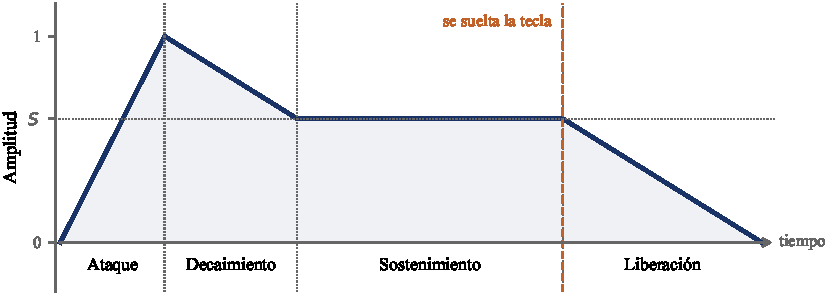
\includegraphics[width=0.85\textwidth]{adsr.pdf}
    \caption{Envolvente ADSR. Los tres primeros tramos dependen de cuánto tiempo
             se mantenga pulsada la tecla; la liberación empieza al soltarla.}
    \label{fig:adsr}
\end{figure}

El otro elemento habitual en la cadena de un sintetizador es el filtro. Un
\gls{lpf} atenúa las frecuencias por encima de una frecuencia de corte, un
\gls{hpf} hace lo contrario, atenúa las frecuencias por debajo de una frecuencia
de corte; y un \gls{bpf} deja pasar únicamente una banda de frecuencia
intermedia. El parámetro de resonancia (Q) realza la respuesta en torno a la
frecuencia de corte, lo que da al filtro buena parte de su carácter sonoro. 

La Figura~\ref{fig:filtros} compara la respuesta en magnitud de los tres tipos
sobre una misma frecuencia de corte.

\begin{figure}[htbp]
    \centering
    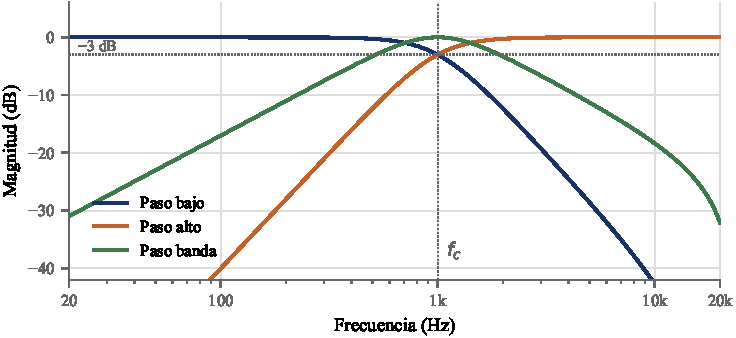
\includegraphics[width=0.85\textwidth]{filtros.pdf}
    \caption{Respuesta en magnitud de un filtro paso bajo, uno paso alto y uno
             paso banda de segundo orden, todos con la frecuencia de corte en
             1~kHz y factor de calidad $Q = 0{,}707$.}
    \label{fig:filtros}
\end{figure}

El orden clásico de la cadena en un sintetizador sustractivo es oscilador, filtro y
amplificador controlado por la envolvente (\gls{adsr}), y es el que se ha mantenido en este
trabajo.

\section{Síntesis por tabla de ondas}

La síntesis wavetable se apoya en una observación sencilla. Si una señal es
periódica, basta con almacenar un único ciclo y repetirlo. En lugar de evaluar
una función trigonométrica para cada muestra, se guarda ese ciclo en una tabla
de $N$ posiciones y se recorre cíclicamente a la velocidad que corresponda a la
nota deseada \cite{BristowJohnson1996}.

El mecanismo que gobierna esa lectura es el acumulador de fase. Se trata de una
variable que avanza una cantidad fija en cada muestra y que vuelve al principio
al llegar al final de la tabla. Siendo $f_0$ la frecuencia de la nota, $f_s$ la
frecuencia de muestreo y $N$ el tamaño de la tabla, el incremento de fase por
muestra es el de la Ecuación~\eqref{eq:incfase}.

\begin{equation}
\label{eq:incfase}
\Delta\varphi = \frac{f_0 \cdot N}{f_s}
\end{equation}

El acumulador avanza según la Ecuación~\eqref{eq:acumulador}, donde el módulo
implementa el retorno al inicio de la tabla al completarse cada ciclo.

\begin{equation}
\label{eq:acumulador}
\varphi[n+1] = \left( \varphi[n] + \Delta\varphi \right) \bmod N
\end{equation}

Como $\Delta\varphi$ no es en general un número entero, el acumulador apunta
casi siempre a una posición intermedia entre dos muestras de la tabla. La
solución habitual es interpolar linealmente entre la muestra anterior y la
siguiente, tal como recoge la Ecuación~\eqref{eq:interplineal}, donde
$i = \lfloor \varphi \rfloor$ y $\alpha = \varphi - i$ es la parte fraccionaria.

\begin{equation}
\label{eq:interplineal}
s[n] = (1-\alpha) \cdot T[i] + \alpha \cdot T[(i+1) \bmod N]
\end{equation}

La Figura~\ref{fig:wavetable} ilustra el proceso completo. El acumulador señala
una posición fraccionaria dentro de la tabla y el valor de salida se obtiene
pesando las dos muestras que lo rodean.

\begin{figure}[htbp]
    \centering
    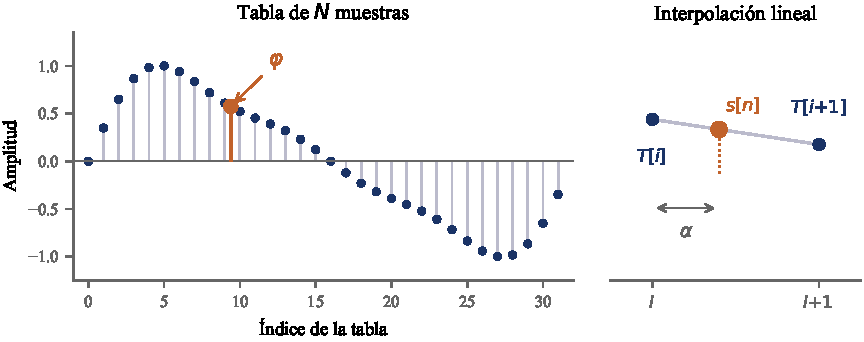
\includegraphics[width=\textwidth]{wavetable.pdf}
    \caption{Lectura de una tabla de ondas. A la izquierda, la tabla almacenada y
             la posición actual del acumulador de fase $\varphi$. A la derecha,
             el detalle de la interpolación lineal entre las dos muestras
             vecinas.}
    \label{fig:wavetable}
\end{figure}

El coste de generar una muestra se reduce así a una suma, dos multiplicaciones y
un acceso a memoria, lo que hace la técnica especialmente adecuada para
microcontroladores. Bristow-Johnson señala además que, para tonos musicales
cuasiperiódicos, este método resulta equivalente a la síntesis aditiva pero
exigiendo mucho menos cálculo en tiempo real \cite{BristowJohnson1996}, que es
justo el compromiso que interesa en un sistema embebido. A cambio, el timbre
queda fijado por el contenido de la tabla, de modo que cambiar de sonido implica
cambiar de tabla.

\subsection{Aliasing y limitación de banda}

Una tabla de $N$ muestras puede contener hasta $N/2$ armónicos. Al reproducirla
a frecuencias altas, los armónicos superiores acaban rebasando la frecuencia de
Nyquist y se reflejan hacia el interior del espectro como componentes de
frecuencia no armónica, audibles como un timbre metálico y desafinado. Este
fenómeno se conoce como \emph{aliasing} y es el principal problema de la
reproducción de tablas a frecuencias elevadas.

La solución habitual consiste en almacenar varias versiones de cada tabla,
filtradas para distintos rangos de nota, y seleccionar en cada momento la que
corresponda al tono que se está tocando \cite{Valimaki2007}. Conviene señalar
que este problema es independiente del tamaño de la tabla y del proceso de
remuestreo empleado para construirla. Aumentar $N$ no elimina el
\emph{aliasing}, solo cambia cuántos armónicos hay disponibles para reflejarse.
Por las razones que se exponen en el capítulo~\ref{cap:diseno}, la limitación de
banda queda fuera del alcance de este trabajo.

\section{Autoencoders y espacio latente}

Un autoencoder es una red neuronal entrenada para reproducir su propia entrada.
Está formado por dos bloques. El codificador transforma la entrada en una
representación de dimensión mucho menor, y el decodificador intenta reconstruir
la entrada original a partir de esa representación. La representación intermedia
recibe el nombre de código o vector latente, y el espacio en el que vive, espacio
latente.

El interés de esta arquitectura no está en la reconstrucción en sí, que sería
trivial si no se impusiera ninguna restricción, sino en el cuello de botella. Al
obligar a que toda la información pase por un número reducido de valores, la red
se ve forzada a descartar lo accesorio y quedarse con los rasgos que de verdad
distinguen unas entradas de otras. Aplicado a un conjunto de formas de onda, el
codificador acaba situando cerca las que comparten características espectrales,
sin que se le haya indicado en ningún momento qué es un armónico.

\subsection{El autoencoder variacional}

Un autoencoder convencional organiza el espacio latente sin ninguna garantía
sobre su estructura. Nada impide que queden zonas vacías entre los puntos
ocupados, y un punto tomado de una de esas zonas puede decodificarse en algo sin
sentido. Para el uso que se pretende aquí, en el que el usuario recorre el plano
con el dedo y pasa continuamente por posiciones que no corresponden a ninguna
onda del conjunto de entrenamiento, esa falta de garantías es un problema.

El autoencoder variacional o \gls{vae} \cite{Kingma2013} resuelve esa limitación
cambiando la naturaleza del código. En lugar de producir un vector de valores
concretos, el codificador produce los parámetros de una distribución de
probabilidad, es decir, un vector de medias $\boldsymbol{\mu}$ y otro de
varianzas $\boldsymbol{\sigma}^2$. El código que recibe el decodificador se
obtiene muestreando esa distribución. Ese muestreo plantea un problema, porque
una operación aleatoria no es derivable y el gradiente no puede atravesarla
durante el entrenamiento. La solución que proponen Kingma y Welling es
reescribir la variable latente como una transformación determinista de la media
y la desviación típica sobre una muestra de ruido tomada aparte, tal como recoge
la Ecuación~\eqref{eq:reparam}. Con esa reformulación, conocida como truco de
reparametrización, la aleatoriedad queda confinada en un término que no depende
de los parámetros de la red, y el gradiente sí puede propagarse.

\begin{equation}
\label{eq:reparam}
\mathbf{z} = \boldsymbol{\mu} + \boldsymbol{\sigma} \odot \boldsymbol{\epsilon},
\qquad \boldsymbol{\epsilon} \sim \mathcal{N}(\mathbf{0}, \mathbf{I})
\end{equation}

A la función de pérdida se le añade además un segundo término que penaliza la
divergencia de Kullback-Leibler entre la distribución producida por el
codificador y una normal estándar. Ese término tira de todas las
distribuciones hacia el mismo punto del espacio, con lo que las zonas ocupadas
se solapan y no quedan huecos. La pérdida total combina entonces el error de
reconstrucción y esa divergencia, como indica la Ecuación~\eqref{eq:vaeloss}.

\begin{equation}
\label{eq:vaeloss}
\mathcal{L} = \underbrace{\mathrm{MSE}(\mathbf{x}, \hat{\mathbf{x}})}_{\text{reconstrucción}}
+ \; \beta \cdot \underbrace{D_{KL}\!\left( q(\mathbf{z}|\mathbf{x}) \,\|\, \mathcal{N}(\mathbf{0},\mathbf{I}) \right)}_{\text{regularización}}
\end{equation}

Para un latente de $d$ dimensiones, la divergencia admite la forma cerrada de la
Ecuación~\eqref{eq:kl}, que es la que se implementa en la práctica.

\begin{equation}
\label{eq:kl}
D_{KL} = -\frac{1}{2} \sum_{j=1}^{d} \left( 1 + \log \sigma_j^2 - \mu_j^2 - \sigma_j^2 \right)
\end{equation}

El factor $\beta$ que aparece en la Ecuación~\eqref{eq:vaeloss} pondera la
importancia relativa de los dos términos y da nombre a la variante conocida como
$\beta$-VAE \cite{Higgins2017}. Higgins y sus coautores lo introducen como un
hiperparámetro que regula el equilibrio entre la capacidad del canal latente y
la precisión de la reconstrucción, y observan que valores mayores que la unidad
empujan al modelo hacia representaciones más ordenadas a costa de reconstruir
peor. Su ajuste supone entonces un compromiso. Valores altos producen un espacio
latente muy regular pero reconstrucciones pobres, porque el modelo prioriza
acercar todas las distribuciones a la normal estándar sobre reproducir fielmente
cada entrada. Valores bajos mejoran la reconstrucción a costa de un espacio
menos continuo.

Existe además un caso degenerado, conocido como colapso posterior, en el que el
modelo opta por ignorar el latente por completo y el término de divergencia se
anula. Bowman y sus coautores se encontraron con este comportamiento al aplicar
un autoencoder variacional a texto, y lo resolvieron introduciendo el peso de la
divergencia de forma progresiva. Durante las primeras épocas el término se anula
o se mantiene muy bajo, de modo que el modelo se centra en aprender a
reconstruir, y solo después se sube hasta su valor definitivo
\cite{Bowman2016}. Es la misma técnica que se ha empleado en este trabajo, tal
como se detalla en el capítulo~\ref{cap:ml}.

\section{Estado del arte}

La aplicación de redes neuronales a la síntesis de audio ha producido en los
últimos años varias líneas de trabajo. Interesa aquí distinguir dos enfoques
distintos según qué es lo que la red genera.

\subsection{Modelos que generan la señal de audio}

Un primer grupo de trabajos emplea la red para generar directamente la forma de
onda de salida, muestra a muestra. El sistema DDSP \cite{Engel2020} combina
elementos clásicos de procesado de señal, como osciladores armónicos y filtros,
con redes neuronales que controlan sus parámetros, de modo que el conocimiento
sobre cómo se genera el sonido queda incorporado a la arquitectura en lugar de
tener que aprenderse desde cero. RAVE \cite{Caillon2021} sigue una vía
diferente. Se trata de un autoencoder variacional entrenado sobre audio en
bruto, con un procedimiento de entrenamiento en dos fases, primero de
aprendizaje de la representación y después de ajuste adversario. Caillon y
Esling añaden un análisis posterior del espacio latente que permite decidir el
compromiso entre fidelidad de reconstrucción y compacidad de la representación,
un problema que aparece de nuevo en este trabajo al fijar la dimensión del
latente. Su interés para este trabajo es que demuestra
que la síntesis neuronal puede alcanzar velocidades de tiempo real, aunque sobre
hardware sensiblemente más potente que un microcontrolador.

\subsection{Modelos que generan tablas de onda}

El segundo grupo, más cercano a lo que se plantea aquí, no genera audio sino
tablas. La red produce una forma de onda de un ciclo que después se reproduce
mediante un oscilador convencional, con lo que el coste de la inferencia queda
desacoplado de la frecuencia de muestreo.

El trabajo de Hantrakul y Yang \cite{Hantrakul2018} es el precedente más
directo. Reutilizan el modelo NSynth WaveNet ya entrenado como autoencoder de
tablas, generando formas de onda de 512 muestras e interpolando entre ellas en
el espacio latente. El resultado se distribuye como \emph{plugin} VST/AU para
estación de trabajo de audio digital.

Dos observaciones suyas resultan especialmente pertinentes aquí. La primera es
de coste. Los propios autores miden unos 4 segundos para codificar y unos 7 para
decodificar una única forma de onda sobre una máquina con GPU, lo que descarta
por completo ejecutar la red durante la reproducción. Su solución fue generar
por adelantado 300 tablas interpolando entre combinaciones de seno, sierra y
triangular, y reproducirlas después con un oscilador convencional. Es exactamente
la misma estrategia que se adopta en este trabajo, y conviene subrayar que allí
la limitación aparece ya sobre una GPU de sobremesa, no sobre un
microcontrolador.

La segunda observación tiene que ver con la estructura del espacio latente.
Hantrakul y Yang comprueban que interpolar a lo largo del segmento que une dos
vectores del espacio produce mezclas utilizables de las dos ondas de partida,
pero que apartarse de ese segmento genera ruido. Dicho de otro modo, en su
modelo no todo el espacio latente es válido, solo lo son las trayectorias entre
puntos conocidos. Para un instrumento en el que el usuario recorre libremente un
plano con el dedo esa garantía no basta, y es una de las razones que justifican
emplear aquí un autoencoder variacional en lugar de uno convencional. Los
propios autores apuntan en esa dirección al plantear como trabajo futuro un
modelo ligero basado precisamente en un autoencoder variacional.

Kreković \cite{Krekovic2021} plantea un oscilador basado en un autoencoder y
estudia el efecto del conjunto de entrenamiento y de los hiperparámetros sobre
la variedad de las formas de onda generadas. Su aportación más pertinente aquí
es la constatación de que emplear las variables latentes directamente como
parámetros de entrada produce una transición suave entre las ondas generadas
cuando los cambios de esos parámetros son pequeños. Es exactamente la propiedad
sobre la que descansa el control táctil de este instrumento.

Más recientemente, Wavespace \cite{Lee2024} propone un generador de tablas
basado en un autoencoder variacional cuyo espacio latente se factoriza por
completo en subespacios asociados a distintos estilos de forma de onda. El
generador se condiciona además con descriptores tímbricos y morfológicos, de
modo que el usuario puede manipular cada subespacio de forma independiente en
lugar de moverse por un plano indiferenciado. Los autores lo prototipan también
como \emph{plugin} de oscilador para estación de trabajo de audio digital, y
señalan que la restricción de velocidad de cálculo sigue siendo el principal
obstáculo cuando se pretende decodificar una forma de onda para cada bloque de
audio.

\subsection{Posicionamiento de este trabajo}

De la revisión anterior se desprende que la generación de tablas de onda
mediante autoencoders y su interpolación en el espacio latente es un problema ya
abordado, y resuelto con solvencia, en varios trabajos previos. La aportación de
este trabajo no está, por tanto, en el modelo.

Lo que ninguno de esos trabajos aborda es la materialización del concepto como
instrumento físico independiente. Todos ellos se presentan como
\emph{plugins}, aplicaciones de escritorio o prototipos de investigación que se
ejecutan sobre un ordenador. La aportación diferencial que se persigue aquí es
la integración embebida completa. Eso supone repartir el sistema entre
microcontroladores de bajo coste, resolver la comunicación entre ellos, mantener
la estabilidad del audio en tiempo real y construir un dispositivo autónomo con
control táctil y entrada \gls{midi} que no necesite un ordenador para funcionar.
El reto no es de aprendizaje automático, sino de ingeniería de sistemas
embebidos.

\chapter{Diseño del sistema}
\label{cap:diseno}

\chapter{Modelo neuronal}
\label{cap:ml}

\chapter{Firmware de control: ESP32-S3 y CYD}
\label{cap:firmware-control}

Este capítulo recorre las dos placas que convierten un dedo apoyado sobre un
cristal en una forma de onda lista para sonar. El reparto de tareas entre
procesadores, la elección del medio de cada enlace y el tamaño de las tramas ya
quedaron justificados en el capítulo~\ref{cap:diseno}, en los
apartados~\ref{sec:arquitectura} y~\ref{sec:enlaces}. Aquí interesa el cómo, es
decir, cómo se lee y se calibra el táctil, cómo se localiza la celda de la
rejilla y se mezclan sus vecinas, cómo se construyen las tramas y cómo se reduce
la onda para dibujarla. Todo lo que sigue corresponde a la fase de ejecución
descrita en el apartado~\ref{sec:fases}, en la que no interviene ninguna red
neuronal.

\section{Lectura y calibración del táctil}
\label{sec:tactil}

La \gls{cyd} es una placa genérica sin manual de fabricante, cuya documentación
es comunitaria \cite{CYDrepo}, así que los pines se confirmaron uno a uno contra
el esquemático que la acompaña. Integra una pantalla \gls{tft} de 240$\times$320
puntos y un táctil resistivo de cuatro hilos gobernado por un XPT2046, que es un
convertidor analógico-digital de aproximaciones sucesivas
(\gls{sar}) de 12 bits \cite{XPT2046}. De ahí sale el dato que gobierna toda la
calibración, y es que cada eje se lee como un entero entre 0 y 4095 en cuentas
del convertidor, sin ninguna relación directa con los píxeles de la pantalla.

Táctil y pantalla cuelgan de buses distintos, y no por casualidad. El táctil usa
el bus VSPI con un objeto propio y los pines de fábrica de la placa, mientras que
la pantalla se controla con la librería \texttt{TFT\_eSPI} \cite{TFTeSPI} sobre
el bus HSPI. Por defecto esa librería también tomaría el VSPI, con lo que dos
objetos acabarían disputándose el mismo periférico. Forzando el HSPI son dos
buses independientes que conviven sin estorbarse, y de paso los pines 12 a 15
son los nativos del HSPI en el ESP32, encaminados por la matriz \mbox{IO MUX}
\cite{EspressifESP32}, que es la ruta directa y rápida. El táctil se lee con la
librería de Stoffregen \cite{XPT2046Touchscreen}.

Esa configuración vive en el fichero de proyecto de PlatformIO y no en el
\texttt{User\_Setup.h} de la librería, que es donde normalmente se pone. El
motivo es práctico. Ese fichero se instala dentro del directorio de dependencias
descargadas, fuera del control de versiones, de modo que la configuración se
perdería al reinstalar la librería o al clonar el proyecto en otro ordenador.
Declarándola como definiciones de compilación viaja con el repositorio. Hay
además un detalle de la placa que conviene no reaprender, y es que la
retroiluminación arranca apagada. La pantalla puede estar pintando
perfectamente y verse negra, indistinguible de un cuelgue, así que se enciende a
mano en la primera línea del arranque. Justo después se dibuja un patrón de
barras de color con un marco, que permite validar el controlador, la orientación
y los colores sin depender todavía del ESP32-S3.

\subsection{De las cuatro esquinas a las dos ventanas}

La primera calibración se hizo tocando las cuatro esquinas del cristal con un
puntero, que al tener un área de contacto pequeña da lecturas más extremas y
limpias que el dedo. De ahí salieron los límites 133 a 3947 en el eje horizontal
y 193 a 3897 en el vertical.

Esos números dejaron de valer cuando la placa se montó girada 180 grados en el
panel, decisión de montaje que se explica en el capítulo~\ref{cap:hardware} y que
busca alejar el conector \gls{usb} de la pantalla \gls{oled}. Al girar la imagen
hay que girar también el táctil, y aquí apareció un hallazgo que ahorró trabajo.
La librería sí aplica la rotación a las lecturas crudas, restándolas de 4095, lo
que evita invertir el mapeo a mano. Pero, por eso mismo, los cuatro límites de
calibración quedan espejados y hay que rehacerlos cruzando mínimo con máximo,
con lo que pasan a 148 a 3962 y 198 a 3902.

La ventana impresa del panel se come parte del cristal, y esa parte hubo que
medirla. La predicción hecha sobre plano, que daba un recorte de 3,75~mm por el
lado izquierdo y nada en vertical, no resistió el banco. Con la placa ya montada,
tocando las cuatro esquinas del hueco, los límites reales salieron 450 a 3730 en
los dos ejes. El labio asimétrico del panel existe, pero pesan más el error de
montaje y un ligero giro del táctil respecto al hueco. Se intentó ajustar esquina
por esquina y se descartó, porque las dos lecturas superiores no coincidían entre
sí en el eje vertical, con unas 230 cuentas de desviación entre la izquierda y la
derecha. Esa discrepancia es la firma de un giro, y un mapeo rectangular no puede
corregir un giro, así que perseguir cuatro números que no cuadran entre ellos
solo habría movido el problema de sitio.

Quedaba un problema más difícil. El labio impreso apoya sobre el cristal en todo
el perímetro y genera pulsaciones fantasma pegadas al borde. Una de las medidas
dio la lectura cruda (3714, 643), a solo 16 cuentas del límite derecho, es decir
dentro del rectángulo que se había dado por útil. Ningún ajuste de esos límites
podía rechazarla sin rechazar también contacto legítimo del dedo. Se probó
entonces a filtrar por presión, aprovechando que el XPT2046 la estima y que el
plástico apoya de forma constante pero floja mientras el dedo aprieta más, y
también se descartó. La fiabilidad de esa lectura en esta placa concreta es
dudosa y, sobre todo, introducía un umbral que mal ajustado podía dejar el táctil
mudo.

\begin{figure}[htbp]
    \centering
    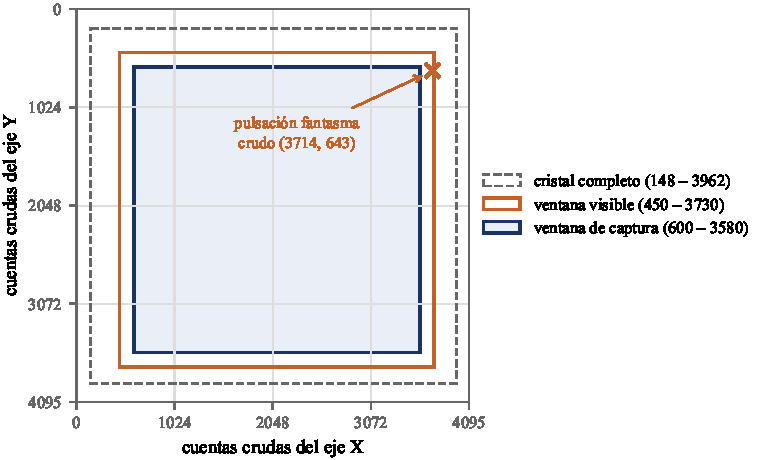
\includegraphics[width=0.70\textwidth]{ventanas.pdf}
    \caption{Las dos ventanas del táctil sobre el plano de cuentas crudas del
             convertidor. La de captura decide qué toques valen y es la que se
             mapea al rango de la coordenada; la visible solo sirve para acotar
             el área de dibujo. La pulsación fantasma medida cae dentro de la
             visible y fuera de la de captura.}
    \label{fig:ventanas}
\end{figure}

La solución fue dejar de usar un solo rectángulo y separar dos, recogidos en la
Figura~\ref{fig:ventanas}. La ventana \emph{visible}, de 450 a 3730, describe lo
que asoma por el hueco y solo se emplea para calcular el área de dibujo. La
ventana de \emph{captura}, de 600 a 3580, decide qué toques se dan por buenos y
deja 150 cuentas de margen por cada lado, unos 2,5~mm. El fantasma medido queda
fuera de ella con 134 cuentas de holgura.

El detalle que hace que esa holgura no cueste nada es cuál de las dos ventanas se
mapea al rango de la coordenada. Se mapea la de captura, no la visible, de modo
que el espacio latente se sigue alcanzando entero de extremo a extremo y lo único
que se pierde son esos 2,5~mm de recorrido del dedo por lado. Mapear la visible
habría dejado las esquinas del plano inalcanzables, que es justamente el defecto
que la recalibración venía a quitar. Y el rechazo es total, no un recorte. La
versión anterior sujetaba la lectura al rango con una función de saturación, así
que un contacto del plástico se enviaba igual, clavado contra el borde del
espacio latente. Ahora un toque fuera de la ventana de captura no genera envío ni
repinta nada, y el instrumento se queda exactamente como estaba.

El táctil se atiende cada 50~ms, sin bloquear el bucle, y solo se envía
coordenada cuando el punto se ha desplazado más de 300 unidades respecto al
último enviado. Como una celda de la rejilla ocupa 4369 unidades del rango de 16
bits, ese umbral es menos de la décima parte de una celda, suficientemente fino
para que el recorrido se perciba continuo y suficientemente grueso para no
saturar el enlace con la vibración de un dedo quieto.

\section{De la coordenada a la celda}
\label{sec:coordenada}

La \gls{cyd} normaliza la lectura al rango de 16 bits antes de enviarla, y esa
decisión tiene una consecuencia comprobada. Ni el giro de 180 grados ni la
recalibración de banco obligaron a tocar una sola línea del firmware del
ESP32-S3, porque este sigue recibiendo el mismo rango de siempre. Resolver el
giro en el procesador de control habría roto la separación de responsabilidades
del apartado~\ref{sec:arquitectura} y habría dejado a la \gls{cyd} enviando
coordenadas que no se corresponden con lo que ella misma muestra.

Del lado del ESP32-S3, la trama de seis bytes descrita en el
apartado~\ref{sec:enlaces} la decodifica una máquina de estados que busca el byte
de cabecera, lee los cuatro de datos y valida la suma de comprobación. Ante
cualquier fallo vuelve al estado inicial a buscar cabecera, de forma que un byte
perdido descuadra una trama pero no el flujo. Conviene señalar que esa entrada
convive con otra por \gls{usb}, en la que la coordenada se escribe a mano como
texto. No es un resto de depuración olvidado. Fue lo que permitió construir y
validar la interpolación antes de que existiera el firmware de la \gls{cyd}, y
es también lo que hace posibles las medidas del capítulo~\ref{cap:pruebas}, que
necesitan una coordenada conocida y estable.

\section{Interpolación bilineal sobre la rejilla}
\label{sec:bilineal}

Localizar la celda es una multiplicación. La coordenada de 16 bits se escala por
$15/65535$, con lo que se obtiene la posición real dentro de la rejilla de
$16\times16$. La parte entera de esa posición da la celda y la parte fraccionaria
da el peso hacia la vecina siguiente. Los dos ejes se tratan de forma
independiente, así que un punto asimétrico no recibe ningún trato especial.

El borde se resuelve sin caso particular. Cuando la coordenada vale el máximo, la
posición escalada da exactamente 15, la vecina de la derecha se sujeta sobre sí
misma y el peso hacia ella queda a cero. La operación sigue siendo la misma
combinación de cuatro tablas, solo que dos de ellas coinciden y aportan peso
nulo, con lo que no se sale del array ni hace falta una rama distinta.

Hay que respetar la convención de índices que fija la cabecera generada en el
apartado~\ref{sec:rejilla}, con la fila recorriendo el eje vertical y la columna
el horizontal. Es el detalle más fácil de equivocar de todo el firmware y el que
peor avisa cuando se equivoca, porque permutar los ejes no rompe nada visible.
La interpolación sigue devolviendo formas de onda perfectamente válidas, solo que
el espacio de timbres queda transpuesto bajo el dedo.

\begin{figure}[htbp]
    \centering
    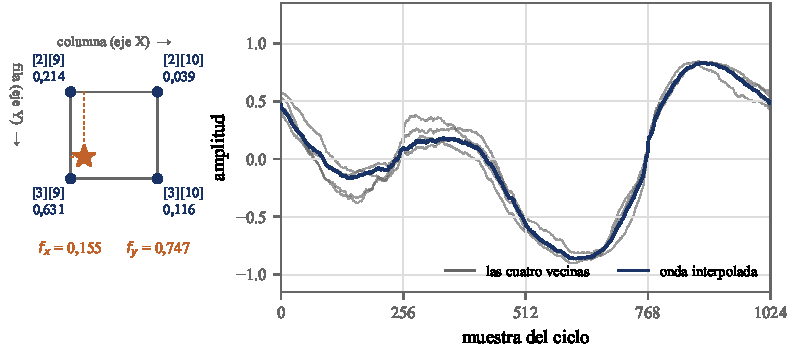
\includegraphics[width=\textwidth]{bilineal.pdf}
    \caption{Interpolación bilineal para la coordenada (40000, 12000). A la
             izquierda, la celda alcanzada, los índices de las cuatro vecinas en
             la rejilla y el peso que recibe cada una. A la derecha, esas cuatro
             formas de onda y la que resulta de mezclarlas.}
    \label{fig:bilineal}
\end{figure}

La Figura~\ref{fig:bilineal} muestra el resultado para la coordenada con la que
después se validó el enlace. Cae en la celda que va de la columna 9 a la 10 y de
la fila 2 a la 3, con pesos de 0,155 y 0,747, de modo que la vecina inferior
izquierda se lleva 0,631 de la mezcla y la superior derecha apenas 0,039. Se
aprecia que la onda resultante no es una de las cuatro ni un promedio simple,
sino que sigue de cerca a la que más pesa.

Merece una aclaración cómo se hace la aritmética, porque el formato de
almacenamiento y el de cálculo no coinciden. Las tablas se guardan como enteros
de 16 bits en formato Q15, pero la mezcla se calcula en coma flotante de 32 bits
y solo se redondea al pasar el resultado a Q15, una vez por muestra. El ESP32-S3
tiene unidad de coma flotante en hardware, así que las mil y pico operaciones que
esto cuesta son despreciables frente a los 1,6~ms que después ocupa la
transferencia, y el cálculo se ejecuta a frecuencia de control, unas decenas de
veces por segundo como mucho. La ventaja de hacerlo así es que cada muestra sufre
un único redondeo en lugar de acumular el de cada paso intermedio. Tampoco hace
falta saturar el resultado, porque los cuatro pesos suman uno y están todos entre
cero y uno, de modo que la mezcla es una combinación convexa de cuatro valores
que ya caben en Q15 y no puede salirse del rango.

La rejilla se compila como una constante de $16\times16\times1024$ enteros de 16
bits, es decir los 512~kB del apartado~\ref{sec:parametros}, y vive en memoria de
programa. En el ESP32-S3 la caché mapea esa memoria al espacio de direcciones, de
modo que se lee como cualquier otro array, sin las macros de acceso que exigen
otras arquitecturas. En memoria de datos solo queda la tabla de trabajo, dos
kilobytes. La \gls{psram} de 8~MB de la placa no llega a intervenir en el camino
principal y queda como margen para la ampliación planteada en el
apartado~\ref{sec:alternativas}.

Para comprobar que esta implementación es correcta no basta con ver que produce
algo. Se escribió una reimplementación independiente en numpy que recalcula la
misma interpolación sobre el fichero de la rejilla y se compara muestra a muestra
con el volcado que el ESP32-S3 imprime por \gls{usb}. Es una comprobación de
equivalencia frente a una referencia, no de plausibilidad. El resultado se recoge
en el capítulo~\ref{cap:pruebas}.

\section{Envío de la tabla al procesador de audio}
\label{sec:emisor-spi}

El ESP32-S3 dispone de varios controladores \gls{spi}, pero dos de ellos quedan
dedicados a la memoria de programa y la \gls{psram} del propio encapsulado y no
son utilizables \cite{EspressifS3}. Se emplea el primero de los de propósito
general, sobre los \gls{gpio} 10 a 13. La elección tenía que esquivar además los
pines que ocupa la variante con memorias octales de esta placa, más el que ya
usaba la entrada del \gls{uart}, y esos cuatro eran los que quedaban libres sin
comprometer nada.

El envío es de maestro, a 10~MHz, en modo 0 y con el bit más significativo por
delante. El selector de chip se gobierna a mano en lugar de dejarlo al
periférico, porque la escritura en bloque de la librería no lo conmuta por su
cuenta. La transferencia de los 2054 bytes bloquea durante 1,6~ms, cosa que no
supone problema alguno a la cadencia de control con la que se llama.

El contenido de la trama es el del apartado~\ref{sec:enlaces}. Las 1024 muestras
se copian en bloque, sin recorrer el array muestra a muestra, porque los dos
extremos del enlace almacenan los enteros de 16 bits en el mismo orden de bytes
y no hay nada que reordenar. Sobre ese bloque se calcula el \gls{crc} de 16 bits
que cierra la trama.

Ese \gls{crc} está escrito tres veces de forma idéntica, en el emisor, en el
receptor y en el guion de validación. Duplicar código suele ser mala señal, pero
aquí es deliberado, ya que tener la misma función en los tres sitios permite
comparar el valor calculado en cada uno y distinguir un fallo de transporte de
un fallo de cálculo. La validación cruzada del enlace tiene una particularidad de
método que conviene contar. El primer intento se hizo deslizando el dedo por la
\gls{cyd}, y resultó inútil, porque con el dedo en movimiento no hay forma de
saber con certeza qué trama recibida corresponde a qué coordenada enviada. Se
repitió con una coordenada fija escrita por \gls{usb}, que es lo que da una
referencia inequívoca. Las cifras están en el capítulo~\ref{cap:pruebas}.

\section{El canal de vuelta y el dibujo de la onda}
\label{sec:pantalla}

Lo que el ESP32-S3 devuelve a la pantalla es dato de representación, nunca de
síntesis. La rejilla y la interpolación siguen viviendo solo en el procesador de
control, y la forma de onda real únicamente sale hacia el procesador de audio por
\gls{spi}. El enlace con la \gls{cyd} ya era bidireccional, así que abrir el
sentido de vuelta no costó más que añadir el hilo y un emisor.

\begin{figure}[htbp]
    \centering
    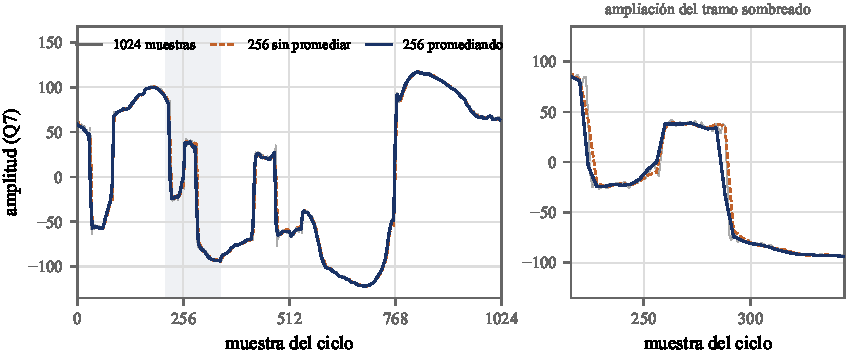
\includegraphics[width=\textwidth]{diezmado.pdf}
    \caption{Reducción de 1024 a 256 puntos para dibujar, sobre el nodo de la
             rejilla en el que más se separan los dos métodos. Promediar cada
             grupo de cuatro muestras y quedarse con una de cada cuatro dan
             prácticamente lo mismo en el grueso del ciclo, y difieren en los
             flancos.}
    \label{fig:diezmado}
\end{figure}

La reducción a 256 puntos de 8 bits, cuyo porqué ya se explicó en el
apartado~\ref{sec:enlaces}, no se hace tomando una muestra de cada cuatro sino
promediando cada grupo de cuatro antes de quedarse con un punto, y el paso de
Q15 a Q7 se resuelve con un desplazamiento de ocho bits.
La Figura~\ref{fig:diezmado} compara los dos métodos sobre el nodo de la rejilla
en el que más se separan. En el grueso del ciclo coinciden, y la diferencia se
concentra en los tramos de pendiente fuerte, donde llega a 68 cuentas de Q7 sobre
una amplitud máxima de 122. Es decir, sin promediar la figura de la pantalla
seguiría reconociéndose, pero colocaría mal los flancos, que es precisamente
donde el ojo juzga la forma de una onda.

Dos tropiezos de esta parte tienen causa identificada y merece la pena dejarlos
escritos. El primero fue que no llegaba ninguna trama buena, no que llegaran
corruptas. El buffer de recepción del puerto serie en esta plataforma es de 256
bytes por omisión, justo por debajo de los 260 que ocupa la trama, y hay que
agrandarlo antes de abrir el puerto. El segundo fue que las tramas se perdían
solo mientras el dedo se movía, que es justo cuando llegan. La causa era una
espera bloqueante en la lectura del táctil, que desatendía la recepción durante
ese tiempo; se sustituyó por una temporización no bloqueante.

El repintado se hace en dos pasadas, borrando entera la traza anterior con el
color de fondo antes de dibujar la nueva. Repintar el área de golpe con un
rectángulo relleno produce parpadeo en cada trama, y borrar e ir pintando de
forma intercalada se come trozos de la línea nueva allí donde las dos se cruzan.
El borrado arrastra también los puntos de la línea central de referencia, que se
repintan sobre la marcha.

Queda el encaje con el panel. Como este tapa un borde del cristal, dibujar sobre
la pantalla completa dejaría parte de la interfaz debajo del plástico, así que el
área útil se acotó a los píxeles que salen de convertir la ventana visible de la
Figura~\ref{fig:ventanas}. Dentro de ella se reparten un título, una banda de
estado con la coordenada, el número de secuencia y el contador de tramas
descartadas, y el recuadro de la onda. La primera versión de ese reparto dejaba
la banda de estado terminando en la misma fila en la que empezaba el recuadro, y
el texto se comía la línea superior del marco. El patrón de arranque cierra el
asunto de forma barata, porque dibuja un marco blanco justo en el límite del área
útil y basta con ver si los cuatro lados asoman por la ventana para saber si las
constantes cuadran con el hueco.

\section{Estado del subsistema}

Con esto queda cerrada la cadena que va del dedo a la trama de audio. La
\gls{cyd} lee el táctil, lo filtra contra la ventana de captura, lo normaliza y
lo envía; el ESP32-S3 localiza la celda, mezcla las cuatro vecinas y entrega la
tabla por \gls{spi}, además de devolver a la pantalla una versión reducida de lo
que está sonando. Las dos comprobaciones cuantitativas que sostienen este
capítulo, la equivalencia de la interpolación frente a la referencia y la
integridad del enlace, se recogen juntas en el capítulo~\ref{cap:pruebas} para
poder leerlas al lado del resto de medidas del sistema montado. Lo que llega al
otro extremo del bus son 2054 bytes cada vez que el dedo se mueve, y qué se hace
con ellos es el asunto del capítulo siguiente.

\chapter{Firmware de audio: Daisy Seed}

\chapter{Hardware y alimentación}
\label{cap:hardware}

Los tres capítulos anteriores describen qué hace cada placa. Este describe el
soporte físico que las sostiene. De dónde sale la energía y cómo se reparte,
sobre qué van montadas, cómo llegan hasta ellas los mandos que el usuario toca
y qué las encierra. El reparto de tareas entre placas está en el
capítulo~\ref{cap:diseno}, la lectura de los canales del panel en el
apartado~\ref{sec:panel} y el tratamiento de las notas en el
apartado~\ref{sec:midi}.

\section{Componentes y equipos}
\label{sec:materiales}

La Tabla~\ref{tab:materiales} recoge los componentes del instrumento. No hay
ninguna pieza fabricada a medida salvo las cuatro piezas de la carcasa, en
línea con el condicionante de partida del apartado~\ref{sec:requisitos}. El
banco de trabajo se reduce a una impresora de filamento con cama de
220$\times$220~mm, una fuente de laboratorio, un soldador y un
multímetro. Los importes se recogen en el anexo de presupuesto.

\begin{table}[htbp]
    \centering
    \caption{Componentes del instrumento.}
    \label{tab:materiales}
    \begin{tabular}{llc}
        \toprule
        \textbf{Bloque} & \textbf{Componente} & \textbf{Cant.} \\
        \midrule
        Módulos
          & Daisy Seed 1.2 & 1 \\
          & CYD ESP32-2432S028R, pantalla táctil de 2,8 pulgadas & 1 \\
          & ESP32-S3 N16R8 & 1 \\
          & Shield \gls{midi} con optoacoplador 6N138 & 1 \\
        \midrule
        Alimentación
          & Alimentador externo de 230~V a 5~V / 3~A & 1 \\
          & Conector de alimentación de 2,1~mm, de chasis & 1 \\
          & Interruptor de encendido ON-OFF-ON & 1 \\
          & Condensador electrolítico de 470~µF, reserva del raíl & 1 \\
          & Condensador electrolítico de 100~µF, filtro de audio & 2 \\
          & Condensador cerámico de 100~nF & 8 \\
          & Resistencia fusible de 3,3~$\Omega$ y 1~W & 1 \\
          & Diodo Schottky 1N5817 & 1 \\
        \midrule
        Panel
          & Potenciómetro lineal de 10~k$\Omega$ & 6 \\
          & Conmutador ON-OFF-ON, selector de filtro & 1 \\
          & Resistencia de 10~k$\Omega$, divisor del selector & 2 \\
          & Pantalla \gls{oled} de 0,96 pulgadas, SSD1306 & 1 \\
          & Jack de audio de 3,5~mm mono, cuerpo de plástico & 1 \\
        \midrule
        Soporte
          & Placa perforada de tiras, 100$\times$160~mm, baquelita & 1 \\
          & Tira de pines hembra de 2,54~mm, 20 contactos & 2 \\
          & Tira de pines hembra de 2,54~mm, 22 contactos & 2 \\
          & Conector JST de 1,25~mm, enlace con la \gls{cyd} & 2 \\
          & Cable de silicona de 24~AWG & --- \\
          & Filamento PLA y tornillería M3 con tuerca & --- \\
        \bottomrule
    \end{tabular}
\end{table}

El teclado que aporta las notas no figura en la tabla. Por la decisión del
apartado~\ref{sec:arquitectura} es un aparato aparte, con su propia
alimentación, y el instrumento funciona con cualquier controlador \gls{midi}.

\section{La alimentación}
\label{sec:alimentacion}
\hypertarget{RE2.2c}{}\label{RE2.2c}

Las cuatro cargas cuelgan en paralelo de un único raíl de 5~V, que es la
tensión de entrada de los tres módulos y del shield, y cada placa regula
internamente sus propios 3,3~V. La Figura~\ref{fig:alimentacion} recoge el
esquema completo.

\begin{figure}[htbp]
    \centering
    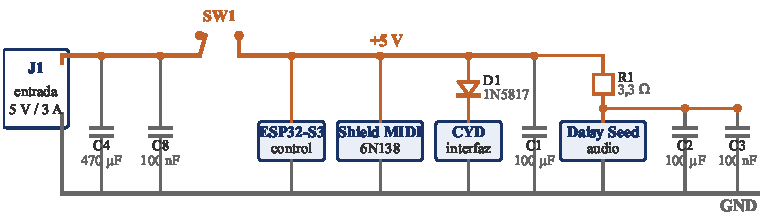
\includegraphics[width=\textwidth]{alimentacion.pdf}
    \caption{Esquema de la alimentación. El condensador de reserva \texttt{C4}
             queda aguas arriba del interruptor y la rama del procesador de
             audio es la única con elemento en serie.}
    \label{fig:alimentacion}
\end{figure}

El consumo del conjunto se estimó en unos 600~mA, de modo que un alimentador de 3~A
deja margen de sobra. Va fuera de la carcasa, así que dentro no hay tensión 
de red en ningún punto. Alimentar todo desde un solo raíl tiene además un tiene además 
un efecto que el UART, el SPI y el MIDI necesitan: las masas de las tres placas quedan 
unidas.

\subsection*{El interruptor y el condensador de reserva}

El raíl no se alimenta directamente desde el conector de entrada. El
electrolítico de 470~µF (\texttt{C4}) queda aguas arriba y el interruptor
aguas abajo, de manera que al cerrar, con el condensador ya cargado, las placas
ven un flanco rápido en lugar de la rampa lenta con la que sube el alimentador.
La razón es que durante esa rampa las placas pasan un tiempo largo en la zona
en la que su circuito de reinicio no sabe decidir, y arrancan de forma
intermitente. Con el flanco rápido y el condensador aportando el pico de
corriente que piden al arrancar el problema desaparece. Para que esto sea
posible el raíl de 5~V deja de ser una tira continua y se corta en un punto,
aguas arriba de todas las cargas, es el interruptor de encendido el que decide cuando
se cierra el circuito y alimenta las cargas. El raíl de masa, en cambio, no se 
interrumpe nunca. Cortarlo obligaría a las corrientes de retorno a buscar camino
por los cables de datos.

\subsection*{Los filtros}

El raíl lo comparten la pantalla y dos microcontroladores conmutando. El ruido que
generan puede acabar en la sección analógica del procesador de audio y salir por el 
jack. Los condensadores de la Figura~\ref{fig:alimentacion} lo atacan aprovechando que
la impedancia de un condensador es un circuito abierto en continua y tiende a un cortocircuito
conforme sube la frecuencia. Este comportamiento se describe con la ecuación \eqref{eq:impedancia}, 
donde $j$ es la unidad imaginaria, $\omega$ la frecuencia angular y $C$ la capacidad del condensador.

\begin{equation}
    Z_C = \frac{1}{j\omega C},
    \label{eq:impedancia}
\end{equation}

Puesto en paralelo con la alimentación, un condensador deriva a
masa la componente de alta frecuencia sin tocar la continua que alimenta las
placas. Por eso el bulk son dos en paralelo y no uno: el electrolítico de
470~µF aporta la capacidad que sostiene los transitorios lentos y el cerámico
de 100~nF es el que es efectivo en la parte alta del espectro.

La rama del procesador de audio lleva además un elemento en serie. La resistencia
\texttt{R1} de 3,3~$\Omega$ junto con los 100~µF de \texttt{C2} forman un paso bajo 
de primer orden cuya frecuencia de corte es la ecuación~\eqref{eq:corte}, que es la 
frecuencia a la que la señal se atenúa 3~dB.

\begin{equation}
    f_c = \frac{1}{2\pi R C} \approx 482~\text{Hz},
    \label{eq:corte}
\end{equation}

De este modo, el ruido de conmutación llega atenuado a la entrada de alimentación 
de la placa. El cerámico \texttt{C3} cubre la parte del espectro que el electrolítico
ya no ve, y va soldado entre las patillas de entrada y de masa del módulo, que son 
adyacentes. Ese elemento en serie no puede ir en el raíl común porque su caída la 
pagarían también las demás cargas. Los parámetros del optoacoplador del shield
están especificados con una alimentación de 4,5~V \cite{Vishay6N138}, que es la
más baja a la que el fabricante garantiza algo, así que sobre un raíl de 5~V el
margen es estrecho para poner nada en serie.
La resistencia elegida es del tipo fusible, es decir, está diseñada para
abrirse ante una sobrecarga. Conviene saberlo porque si se abre, la placa de audio 
deja de recibir alimentación y el instrumento queda mudo.

\subsection*{El diodo de la rama de la pantalla táctil}

La \gls{cyd} se reprograma por su propio conector \gls{usb}, así que en algún
momento va a estar alimentada por las dos fuentes a la vez. El diodo Schottky
\texttt{D1} en su rama resuelve el conflicto. La placa toma la más alta de las 
dos fuentes, así la caída del Schottky sería suficiente para que la \gls{usb} predomine.
Se elige Schottky por su caída directa baja, del orden de tres décimas de
voltio, que sobre un raíl de 5~V es asumible. Los otros dos módulos llevan ese
diodo integrado y no lo necesitan.

\subsection*{Las masas}

El fabricante del procesador de audio exige unir la masa analógica con la
digital en toda aplicación \cite{DaisySeed}, y esa unión se hace en un único
punto y cerca de la placa. Conviene precisar qué significa eso, porque unidas en
un punto las dos masas son el mismo nodo y a corriente continua están al mismo
potencial. Lo que las distingue no es el nodo sino el camino: el cobre que
separa cualquier punto de masa del punto de unión tiene resistencia, y por él
circula la corriente de retorno de lo que haya aguas arriba. Medido sobre la
placa, entre una y otra masa hay unos 1,7~mV.

De ahí salen las dos decisiones de trazado. El manguito del jack se lleva a la
patilla de masa analógica y no al raíl general, para que el retorno de la salida
de audio no comparta cobre con el de los dos microcontroladores. Los
potenciómetros, en cambio, se referencian a la masa digital, que quedaba mucho
más a mano en el trazado, porque 1,7~mV sobre un fondo de escala de 3,3~V son un
0,05\,\% y no mueven una lectura de mando. La patilla superior sigue colgando de
la alimentación analógica, así que la cancelación que se explicó en el
apartado~\ref{sec:panel} queda intacta.

\section{Diseño del circuito y trazado de la placa}
\label{sec:veroboard}

El montaje definitivo va sobre una placa perforada de tiras de cobre de
100$\times$160~mm, que a paso de 2,54~mm son 39 tiras de 63 agujeros cada una.
El circuito se dibujó en Fritzing sobre su vista de placa de tiras, que es a la
vez esquema y plano de montaje. En una placa de este tipo la posición de
cada componente forma parte del circuito. El resultado es la
Figura~\ref{fig:fritzing}. Sobre ese fichero se verificó el trazado
decodificándolo hueco a hueco.

\begin{figure}[htbp]
    \centering
    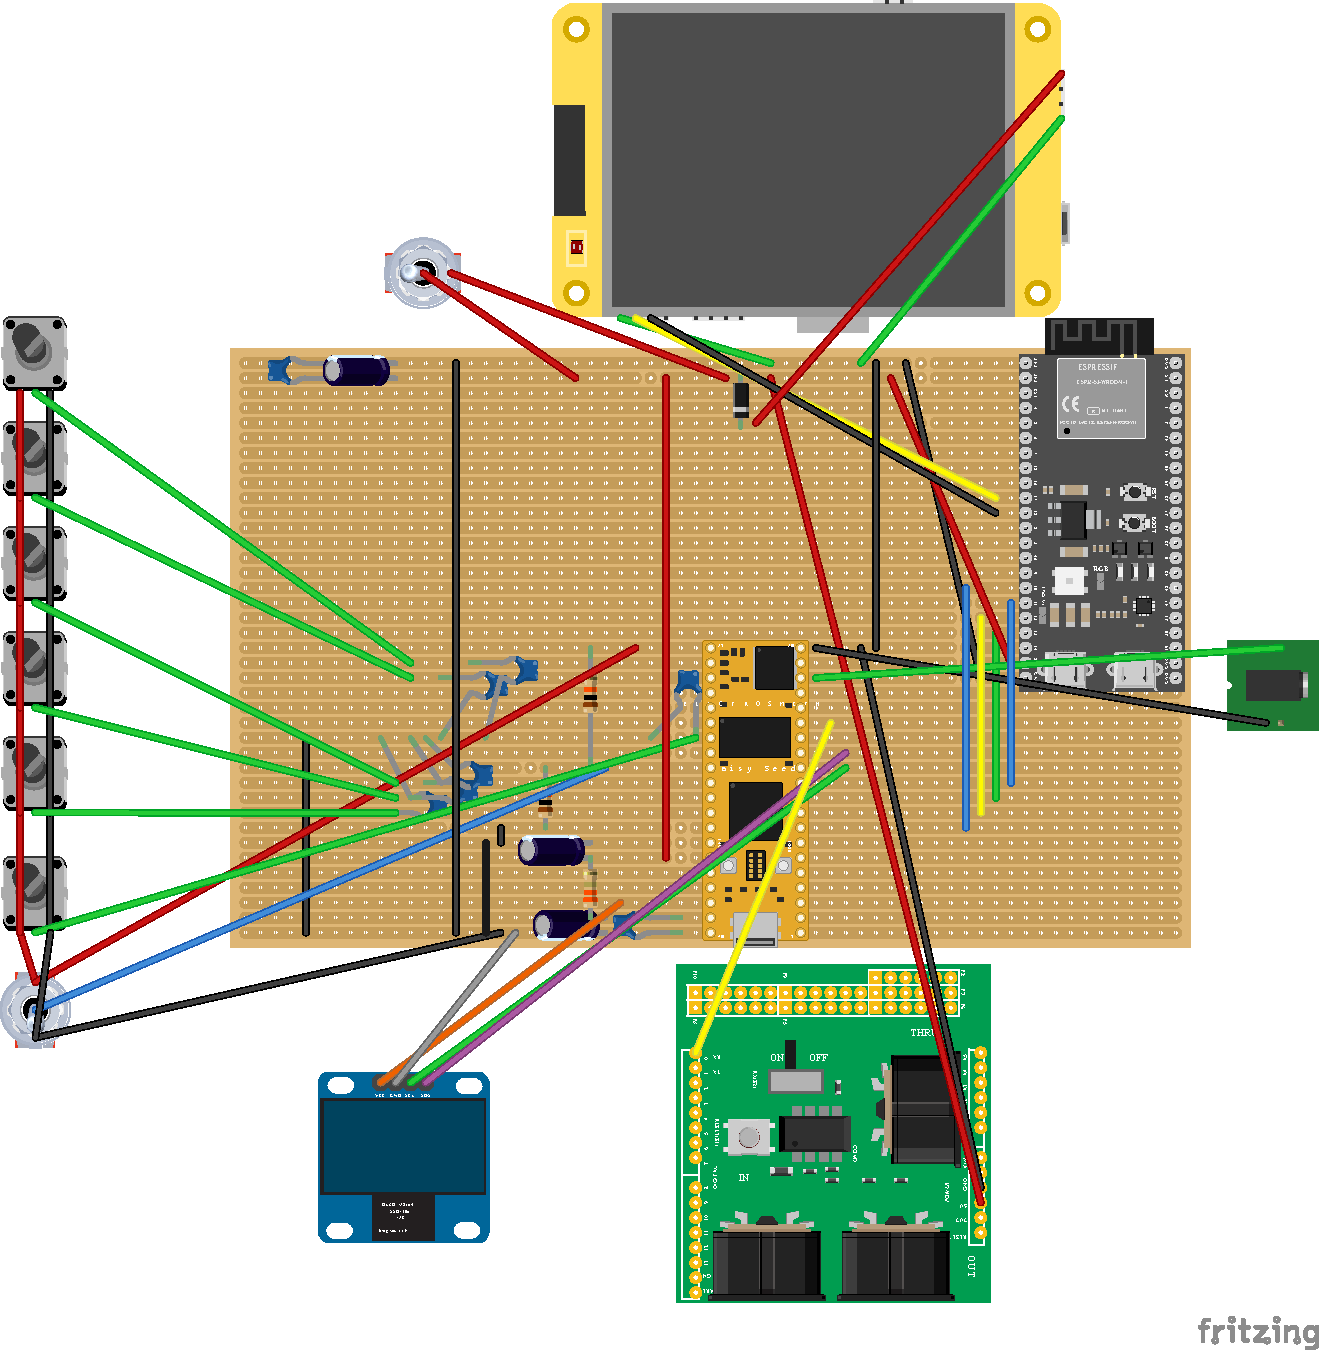
\includegraphics[width=0.86\textwidth]{fritzing_veroboard.pdf}
    \caption{Trazado de la placa. Los dos módulos van sobre zócalos, la
             alimentación ocupa el extremo libre de los raíles y todo lo que el
             usuario toca sube al panel por el mazo.}
    \label{fig:fritzing}
\end{figure}

\subsection*{Los cortes de pista}

Un módulo con dos filas de
patillas, colocado perpendicular a las tiras, deja enfrentadas la patilla $p$ y
la $41-p$ sobre la misma tira, y por tanto en cortocircuito. Colocarlo paralelo
no es la solución, porque entonces las veinte patillas de una fila caen sobre
la misma tira. Hay que cortar, por tanto, las tiras que pasan bajo las placas. 
Hay que llevar especial cuidado con cinco de esas uniones ya que son destructivas 
si se olvidan. La peor pone la alimentación analógica directamente contra la masa
analógica, otra mete los 5~V de la entrada de alimentación en una \gls{gpio} y una tercera 
deja el cursor de un potenciómetro sobre la salida de audio.

Tras hacer los agujeros se comprueban con doble medida. Una a lo largo de la tira
cruzando el agujero, que tiene que quedar en abierto, y otra contra las dos tiras
vecinas, por si la broca ha raspado el borde. De hecho, gracias a la segunda medida 
se cazó una rebaba de cobre que había creado un cortocircuito.

\subsection*{Reparto de la placa}

Para la disposición en la placa se tomaron unos acuerdos.
La tira 1 es el raíl de masa y la tira 2 el de 5~V. El reparto a lo largo de
los 63 agujeros se hizo por naturaleza de la señal. El enlace \gls{spi} corre a
10~MHz, por lo que es la señal más agresiva de la placa y sus flancos se
acoplan con facilidad a lo que tenga cerca. Por este motivo su recorrido tiene
que ser corto y no pasar cerca del jack ni de los cursores.
Mientras que la salida de audio y la masa analógica se van al borde opuesto,
donde además caen las patillas de los potenciómetros. Así se acaba creando una zona
digital, una mixta y una analógica, y la sección de alimentación en el extremo libre
de los raíles, que es donde la obliga a estar el corte del interruptor.

Conviene subrayar que esta placa no es «el circuito» sino un «concentrador».
Los dos módulos sobre zócalos, la alimentación con su filtro y una fila de 
conexiones. Nada de lo que el usuario toca o mira va soldado a ella. Todo eso 
vive en el panel y baja por cables a la placa, como en un pedal de guitarra.

El trazado se calcó sobre la cara de cobre en lugar de sobre la de baquelita, y
como la vista de la herramienta es la cara de componentes, la placa salió en
espejo respecto al diseño. Con los cortes ya taladrados se optó por adaptarse a la
placa y volver a trazar esta vez contando sobre la baquelita. Por este motivo, en la placa
se pueden visualizar cortes de pista que no son necesarios y otros que sí lo son. 
La Figura~\ref{fig:fritzing} es la versión final. El cambio, además, obligó a reasignar
tres cursores y el selector de filtro a otras patillas.

\section{El panel de control}
\label{sec:panel-fisico}

La Figura~\ref{fig:panel} es el alzado del panel, dibujado a escala a partir
del mismo fichero paramétrico del que salió la pieza impresa.

\begin{figure}[htbp]
    \centering
    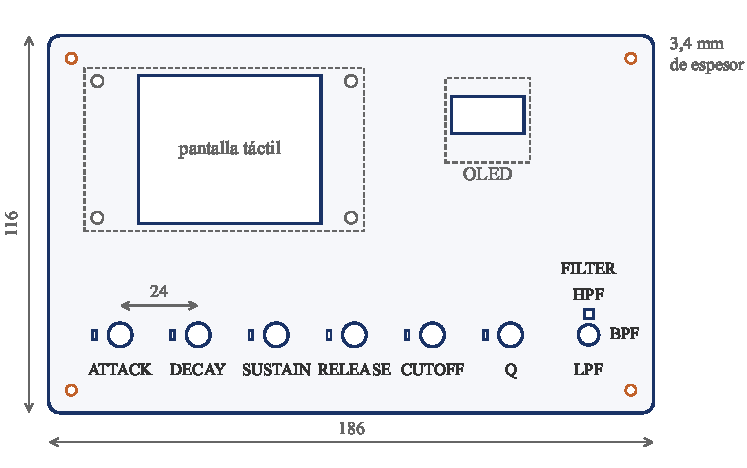
\includegraphics[width=0.72\textwidth]{panel.pdf}
    \caption{Alzado del panel frontal. El trazo discontinuo es el contorno de
             las dos placas, que quedan por detrás; el continuo, lo que se ve
             desde fuera. Cotas en milímetros.}
    \label{fig:panel}
\end{figure}

Los seis potenciómetros son lineales de 10~k$\Omega$ y cuelgan de la
alimentación analógica del procesador de audio, que es la disposición que el
fabricante recoge como aplicación típica \cite{DaisySeed}. El valor hace que
los seis sumen unos 2~mA de consumo sobre el raíl analógico. Mientras
que un valor menor lo cargaría sin motivo, valores mayores harían la lectura más
sensible al ruido captado por el cable. Cada cursor lleva un cerámico de 100~nF
a la masa, soldado en el extremo de la placa para poder filtrar lo que 
ha recogido el hilo. Las dos resistencias de 10~k$\Omega$ del divisor del selector,
cuya función se explicó en el apartado~\ref{sec:panel}, van también en la placa, 
así que al panel sólo llega un hilo de cada potenciómetro y uno del selector. La 
alimentación 3V3 analógica y la masa van en daisy chain, desde el selector hasta el 
último potenciómetro, y de ahí a la placa. 

Para el grosor del panel se tomó en cuenta la rosca del potenciómetro, que mide
7,0~mm, de la que hay que descontar arandela y tuerca. De esta manera, el máximo
que podía medir el panel de grosor eran 4,1~mm pero se optó por 3,4~mm porque era
más que suficiente. Se decidió también añadir el hueco para la patilla antigiro de
cada potenciómetro, que no es redonda sino una pletina rectangular de
2,8 por 1,2~mm, y que se corta pasante como el propio agujero de la rosca. Es
lo que impide que el cuerpo del potenciómetro gire dentro del panel al mover el
mando, con la tuerca limitándose a apretarlo contra la plancha.

Una parte complicada fueron las ventanas para las pantallas montadas en el panel.
La ventana de la \gls{cyd} lleva el labio izquierdo cuatro milímetros más adentro 
que el derecho para tapar un borde negro que asomaba. El labio, que apoya sobre el 
cristal en todo el perímetro, fue una fuente de pulsación fantasma como se comentó 
en el apartado \ref{sec:tactil}. Además, la pantalla va girada media 
vuelta por un motivo físico, que su conector \gls{usb} quede en el lado opuesto a la 
\gls{oled}. Esto hizo que se tuviera que rehacer parte de su firmware y recalibrarla 
entera, está descrito en el apartado~\ref{sec:tactil}.
La \gls{oled} se resolvió en tres niveles. Uno para el asiento de la placa, otro para
el hueco del cristal y un labio para acotar la parte visible de la pantalla con un canal 
para que su cable plano no quede pinzado. 

Para las etiquetas, se decidió que fuesen grabadas con un milímetro de
profundidad y que su tamaño se ajustase solo según el número de caracteres, para que
las largas no invadan a sus vecinas.

Fuera del panel quedan el jack, los conectores \gls{midi}, la entrada de
alimentación y el interruptor de encendido, que se llevaron a las paredes de la caja.

\section{La carcasa}
\label{sec:carcasa}

La carcasa no es una pieza de forma arbitraria, es un conjunto de agujeros a cotas
exactas y cada cota depende de una pieza física que hay que medir. Para solucionar esto, se
modeló con una herramienta de diseño paramétrico por texto, en la que corregir
una cota es cambiar un número, en lugar de con un modelador orgánico, donde
habría que rehacer la geometría. El método de trabajo fue ir imprimiendo probetas 
que comprueban si las cotas son correctas poco a poco. La probeta debía laminarse con el
mismo perfil que la pieza definitiva, ya que el diámetro real de un agujero
impreso depende de factores de la impresión como el ancho de línea, el número de perímetros 
o de la velocidad de impresión. Por eso la probeta se implementó dentro del propio fichero 
de la pieza, seleccionable con un parámetro, de modo que comparte parámetros con ella. 
Las probetas ayudan a depurar el modelo y a calibrar la impresora reduciendo el
tiempo de prueba y error y el desperdicio de filamento. La Figura~\ref{fig:carcasa} muestra 
la carcasa montada y despiece.

El cuerpo es una cuña de 44~mm de alto por delante y 62 por detrás, lo que deja
la cara inclinada a algo menos de nueve grados. Tiene una bahía trasera plana que
lleva la planta a 186 por 186,6~mm, y está partido en tres piezas, como muestra
la Figura~\ref{fig:carcasa}. Cada pieza se imprime en la orientación en la
que su geometría queda vertical o apoyada para minimizar el uso de soportes y para
ser más preciso con los contornos críticos. Por ejemplo, al imprimir la trasera tumbada sobre su cara exterior,
los huecos de los conectores \gls{midi} se convierten en agujeros verticales pasantes.
Así desaparecen a la vez los voladizos y los puentes de impresión que habrían empeorado
la precisión de la pieza.

Todas las uniones son por tornillo contra tuerca metálica embutida y ninguna con
rosca en el plástico. El material del que está impreso, PLA, no aguanta bien las 
fuerzas de rosca y puede deshacerse con el tiempo. Además, para todos los agujeros se 
crearon parámetros de holgura editables. Estos valores de holgura vendrán dados por lo
comentado anteriormente, probetas y configuraciones de la impresora. De hecho, los
agujeros impresos salen entre 0,2 y 0,35~mm menores que la cota real puesta en el modelo, 
así que, por ejemplo, los pasos de tornillo de 3~mm van dibujados entre 3,4 y 3,8.

La Figura~\ref{fig:instrumento} muestra el instrumento terminado, ya montado y
en funcionamiento.

\begin{figure}[H]
    \centering
    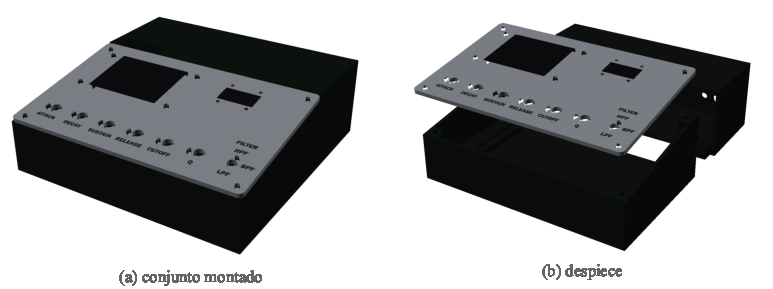
\includegraphics[width=\textwidth]{carcasa.pdf}
    \caption{La carcasa, renderizada desde el modelo paramétrico. A la
             izquierda el conjunto montado; a la derecha el despiece, con el
             panel separado de la bandeja y las dos piezas de la trasera.}
    \label{fig:carcasa}
\end{figure}

\begin{figure}[H]
    \centering
    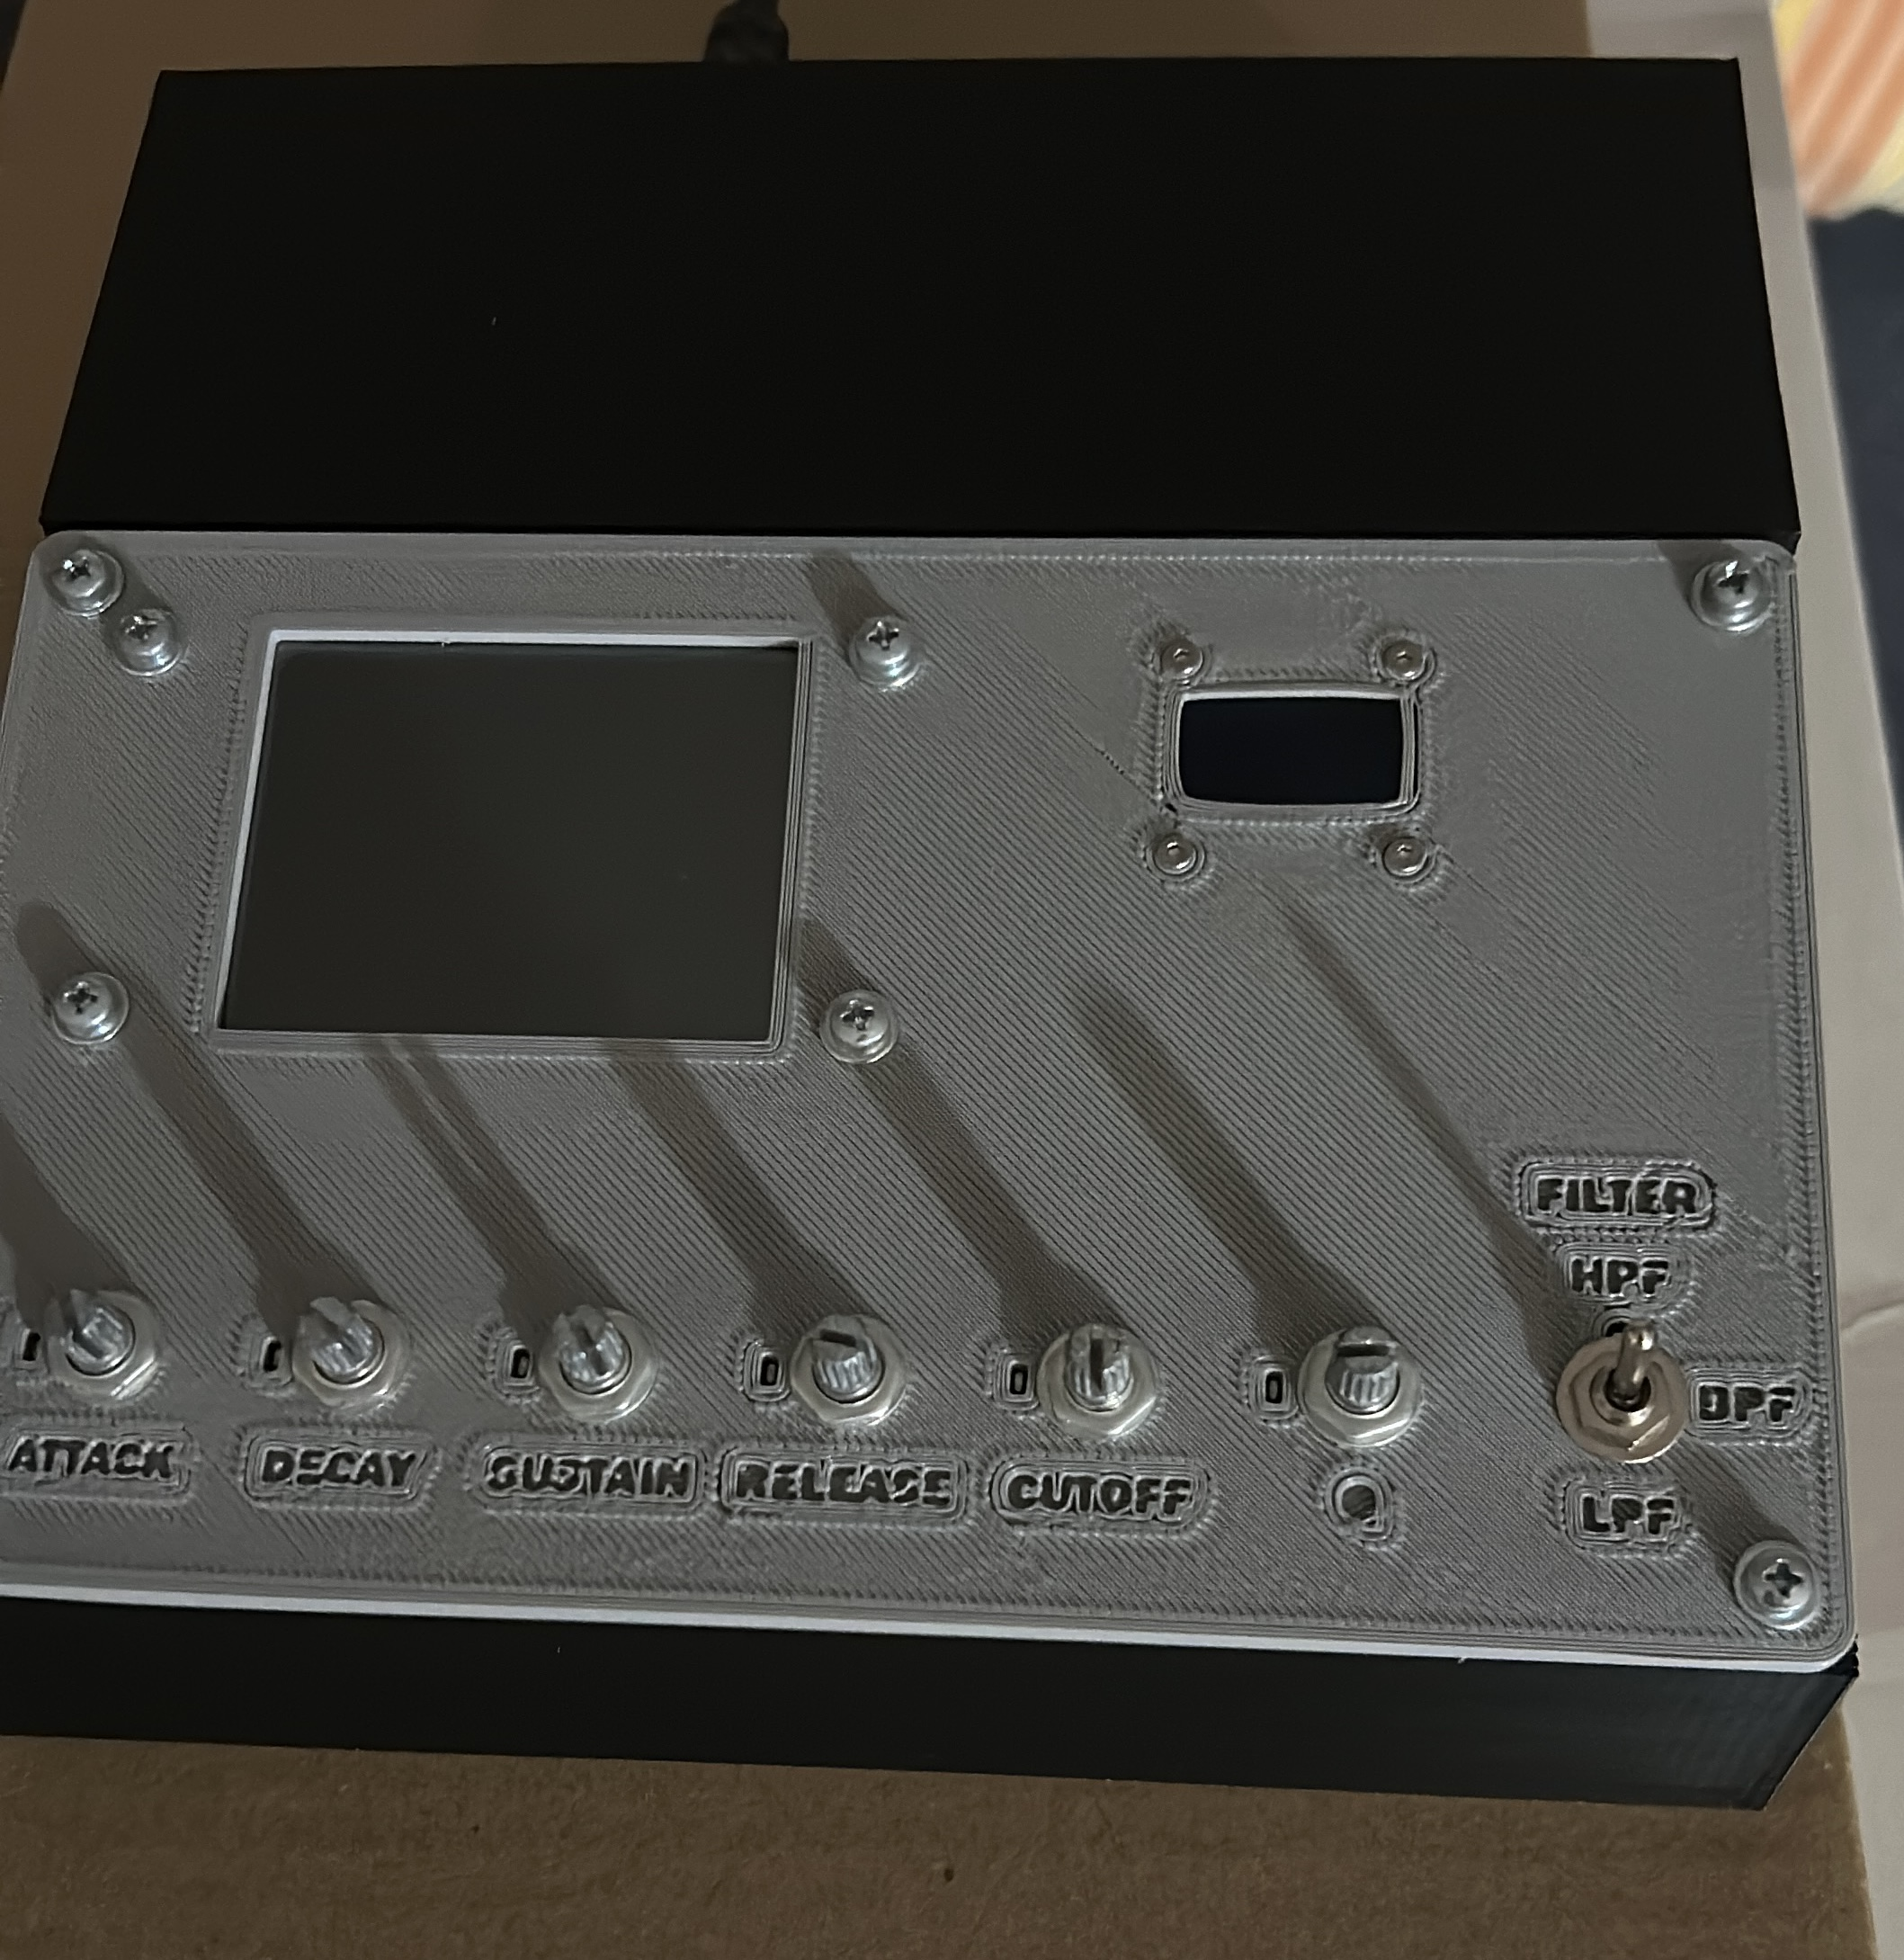
\includegraphics[height=7.5cm]{instrumento_panel.jpg}\hfill
    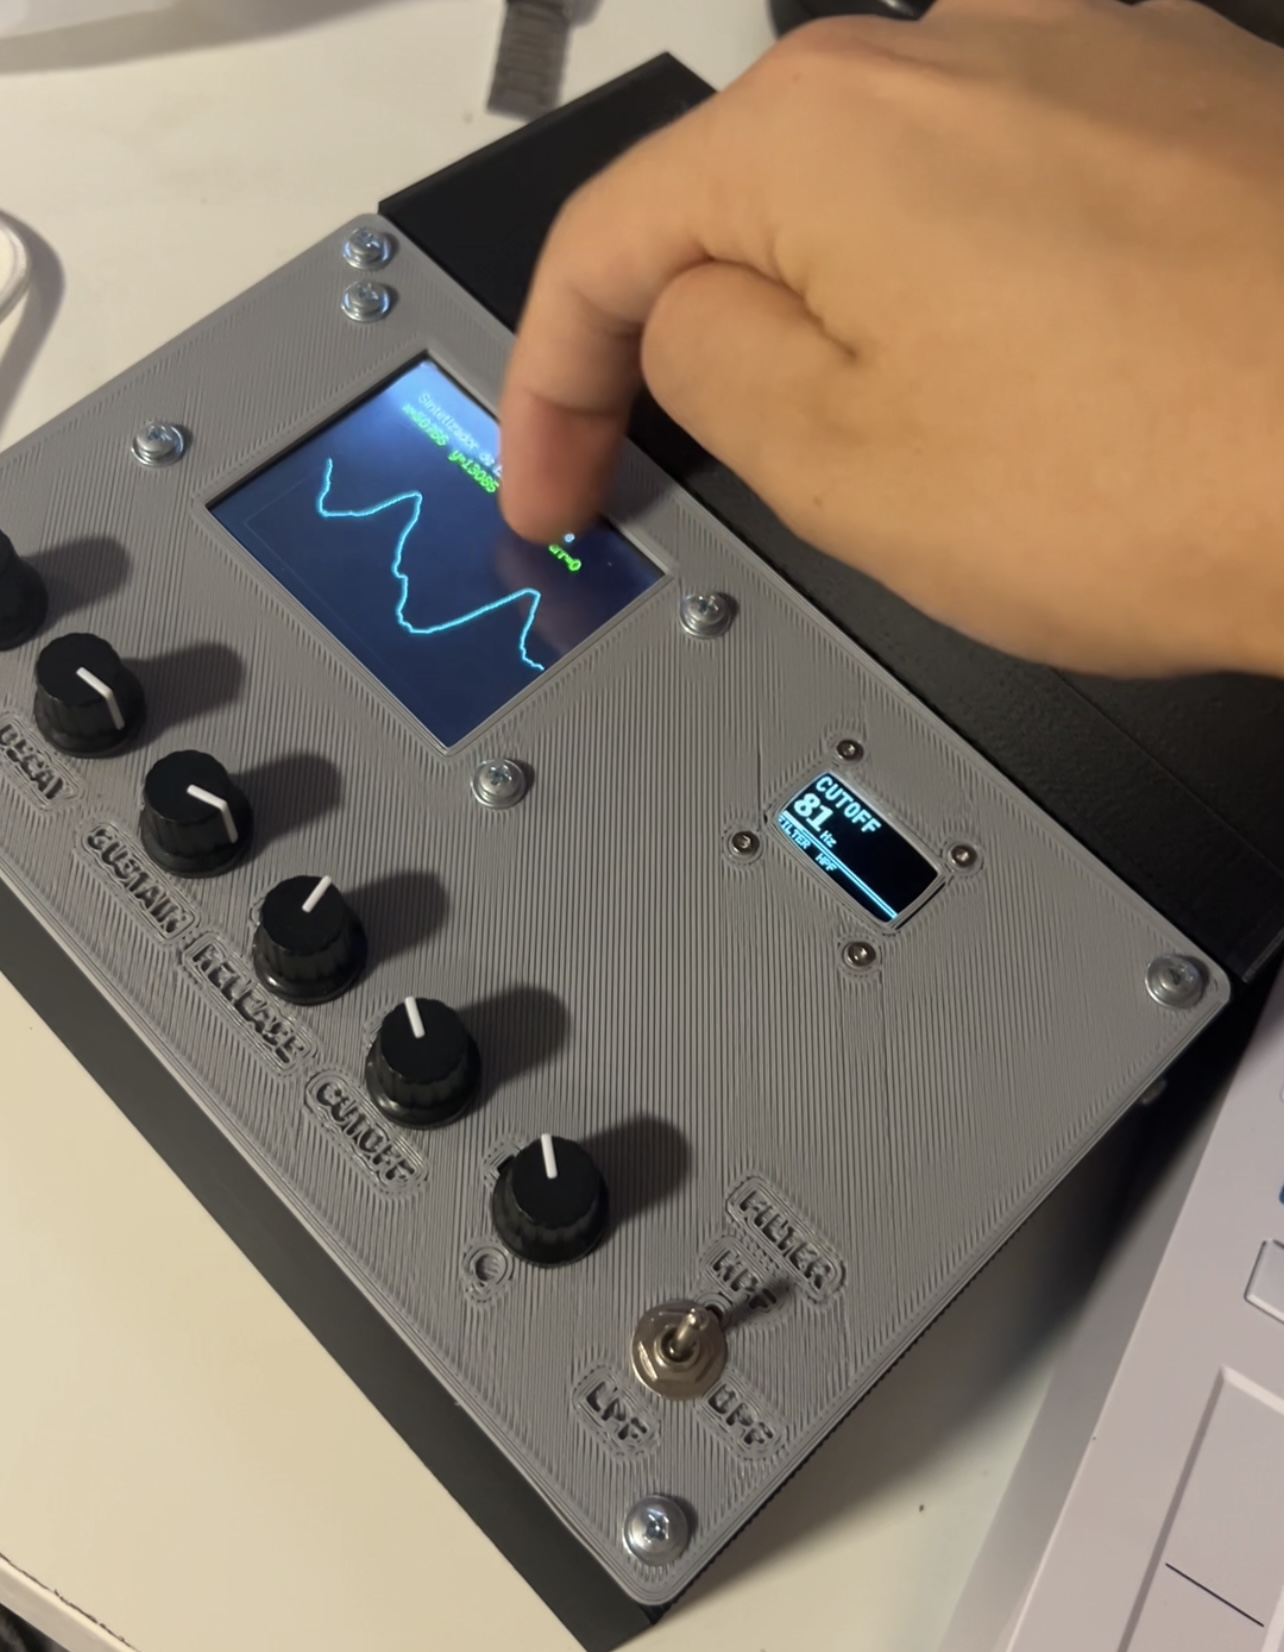
\includegraphics[height=7.5cm]{instrumento_uso.jpg}
    \caption{El instrumento terminado. A la izquierda, el panel de control con
             los seis mandos, el selector de tipo de filtro y los huecos de las
             dos pantallas. A la derecha, en funcionamiento: el dedo fija el
             punto del espacio latente, la pantalla táctil dibuja la forma de
             onda que se genera en ese punto y el display de servicio muestra
             el parámetro que se está editando.}
    \label{fig:instrumento}
\end{figure}

Con la caja montada, el instrumento queda descrito por completo, del conjunto
de datos al plástico. Queda pendiente la comprobación eléctrica sobre la placa
ya soldada, que debe cerrar la cuestión de la tensión de entrada del procesador
de audio, y queda comprobar que el conjunto hace lo que se dice que hace, que
es el asunto del capítulo siguiente.

\chapter{Pruebas y resultados}
\label{cap:pruebas}

\chapter{Conclusiones y trabajo futuro}
\label{cap:conclusiones}

\section{Síntesis y aportación del trabajo}
\hypertarget{RE3.2}{}\label{RE3.2}

El trabajo entrega una cadena completa y cerrada, que empieza en un conjunto
público de formas de onda y termina en una señal de línea en un conector de
3,5~mm. Entre esos dos extremos hay un autoencoder variacional entrenado en el
ordenador, una rejilla de 256 tablas horneada a partir
de su decodificador, tres microcontroladores con una responsabilidad única cada
uno, dos enlaces de datos verificados muestra a muestra y una carcasa que lo
alberga todo. El reparto que hace posible ese encadenamiento se describe en el
apartado~\ref{sec:arquitectura}. Lo que ese conjunto demuestra es que un espacio
tímbrico aprendido se puede recorrer con el dedo sobre hardware de catálogo, con
83,82~euros de materiales según el Apéndice~\ref{anx:presupuesto}, sin un
ordenador delante y sin ningún circuito integrado hecho a medida.

Conviene dejar dicho con precisión qué papel juega aquí el aprendizaje
automático, porque es donde más fácil resulta exagerar. En el instrumento no se
ejecuta ninguna red neuronal. El codificador solo intervino durante el
entrenamiento y el decodificador se ejecutó fuera de línea para hornear la
rejilla, de modo que en marcha solo hay consulta de tabla e interpolación. La
inteligencia está en el contenido de las tablas y no en el código que las lee,
ya que el hecho de que celdas vecinas suenen emparentadas y de que cruzar el
plano produzca una transición tímbrica coherente es producto del latente
aprendido y no se obtiene a mano. Precalcular fue una estrategia de despliegue y
no una renuncia, y el motivo está en el tiempo de cálculo y no en el espacio,
tal como se razonó en el apartado~\ref{sec:alternativas}. El tamaño de memoria, de hecho,
no distinguía entre las dos opciones. La rejilla ocupa 512~kB
(apartado~\ref{sec:rejilla}) y el decodificador, con sus cerca de 592.000
parámetros, ocuparía del orden de 590~kB cuantizado a ocho bits. Lo que la
rejilla compra es un coste de acceso constante y conocido. Lo que paga a cambio
es una resolución del plano congelada en el momento de hornearla.

\section{Cumplimiento de los objetivos}
\hypertarget{RE3.1}{}\label{RE3.1}

Los tres primeros objetivos específicos corresponden a la fase de preparación y
quedan cumplidos. El conjunto de datos homogéneo se construyó resolviendo el
remuestreo, la normalización de amplitud y la alineación de fase
(apartado~\ref{sec:preprocesado}). El autoencoder variacional comprime cada onda
a una coordenada de dos dimensiones, y su plano resultó continuo y bien
aprovechado (apartado~\ref{sec:latente}), con la diversidad confirmada después
sobre la propia rejilla (apartado~\ref{sec:demo}). Y esa rejilla se horneó y se
exportó en un formato que el firmware compila directamente
(apartado~\ref{sec:rejilla}).

Los tres siguientes son de firmware y también quedan cumplidos. El motor
sustituye la tabla en reproducción sin discontinuidad audible, con una
transición cuyo rizado de pico se midió en 0,34~dB
(apartado~\ref{sec:crossfade}). La comunicación entre las tres placas quedó
definida y verificada, con la interpolación equivalente a su referencia dentro
de 1~\gls{lsb} y el transporte por \gls{spi} sin una sola muestra alterada
(apartado~\ref{sec:validacion-datos}). El control de nota y dinámica por
\gls{midi} funciona, con las 128 notas dentro de tolerancia y el la central en
440~Hz sobre el montaje definitivo, y el panel analógico recorre el fondo de
escala completo en todos sus canales (apartado~\ref{sec:tensiones}). Este último
objetivo se cumple con una salvedad que no conviene disimular, y es que la
realimentación visual de los mandos no llegó a funcionar sobre el aparato
montado (apartado~\ref{sec:incidencias}).

Quedan el objetivo de validar cada etapa contra una referencia calculada en el
ordenador, que atraviesa todo el desarrollo y se recoge reunido en el
capítulo~\ref{cap:pruebas}, y el de integrar el conjunto en un prototipo físico
alimentado desde una fuente única, que consume 0,42~A y entrega 198,7~mV
eficaces de nivel de línea (apartados~\ref{sec:consumo} y~\ref{sec:audio}).
También este último lleva salvedad, y es que el procesador de audio trabaja
medio voltio por debajo de la tensión de entrada mínima que garantiza su
fabricante, con la causa identificada y la corrección propuesta
(apartado~\ref{sec:balance}). Con esas dos salvedades sobre la mesa, el objetivo
general se considera alcanzado. Hay un instrumento autónomo que permite explorar
un espacio tímbrico aprendido con una pantalla táctil y una entrada \gls{midi}
estándar.

\section{Aprendizajes del proyecto}

Por encima de cualquier resultado concreto, el trabajo ha permitido aplicar
sobre un mismo objeto contenidos que en el grado se estudian por separado. El
aprendizaje automático entrena el modelo, el procesado de señal prepara las
ondas y las reproduce, los sistemas embebidos reparten la carga entre tres
procesadores, la electrónica analógica resuelve el panel y la alimentación, los
protocolos de comunicación unen las placas y el diseño mecánico las encierra en
algo que cabe en las manos. Que todas esas materias tuvieran que encajar en un
único aparato, y no cada una en su práctica, ha sido lo más satisfactorio del
proyecto, y es la razón por la que se eligió este tema y no otro más acotado.

\section{Trabajo futuro}
\hypertarget{RE3.2b}{}\label{RE3.2b}

Las líneas de continuación salen todas de una limitación conocida, y conviene
enunciarlas con ella delante. La primera es la que el capítulo~\ref{cap:diseno}
dejó abierta a propósito. El decodificador puede llegar a ejecutarse a bordo del
ESP32-S3, y el reparto elegido lo permite sin tocar el firmware del procesador
de audio, que seguiría recibiendo exactamente lo mismo
(apartado~\ref{sec:alternativas}). Antes de intentarlo conviene saber si merece
la pena, y esa comprobación no necesita hardware. Como el decodificador no es
lineal, interpolar entre dos de sus salidas no equivale a decodificar el punto
latente intermedio, de modo que comparar ambas cosas en puntos intermedios daría
la cifra de error de aproximación que hoy no existe, y con ella se sabría si una
rejilla de $16 \times 16$ basta. La segunda línea es la limitación de banda de
las tablas, que quedó fuera del alcance porque corregirla multiplica el volumen
de datos embarcado por el número de versiones filtradas que haya que almacenar
(apartado~\ref{sec:parametros}), y que se resolvería eligiendo la adecuada según
el registro de la nota. La tercera es la fidelidad del cuello de botella de dos
dimensiones, que redondea los flancos verticales
(apartado~\ref{sec:reconstruccion}) y cuya ampliación obligaría a replantear el
control táctil, que es precisamente lo que fijó esas dos dimensiones.

Antes que ninguna de ellas está la revisión del propio aparato. Las tres
incidencias que la verificación dejó abiertas siguen abiertas
(apartado~\ref{sec:incidencias}). Falta además levantar con
osciloscopio y analizador lo que un multímetro no alcanza, esto es, la
distorsión, la respuesta en frecuencia y el pico de corriente del arranque
(apartado~\ref{sec:balance}). La polifonía, descartada desde el principio, solo
tiene sentido plantearla cuando todo lo anterior esté resuelto.

El prototipo es lo más perecedero de todo esto. Lo que permanece no está dentro
de la caja, sino dentro de mi cabeza. La experiencia de haberlo hecho, de haberlo 
pensado y de haberlo escrito es lo que queda, y es lo que me permitirá abordar con
más seguridad los próximos proyectos. Proyectos serán más ambiciosos, proyectos que espero que me dejen
con la misma sensación de haber aprendido algo que no estaba en ningún libro ni en ninguna clase. 



%%%%%%%%%%%%%%%%%%%%%%%%%%%%%%%%%%%%%%%%%%%%%%%%%%%%%%%%%%%%%%%%%%%%%%%
%%%%%%%%%%%%%%%%%%%%%%%%%%%%%%%%%%%%%%%%%%%%%%%%%%%%%%%%%%%%%%%%%%%%%%%
\printbibliography[heading=firstlevel,title=Bibliografía]
%\addcontentsline{toc}{chapter}{Bibliografía}
\label{sec:biblio}
\newpage\thispagestyle{empty}
%%%%%%%%%%%%%%%%%%%%%%%%%%%%%%%%%%%%%%%%%%%%%%%%%%%%%%%%%%%%%%%%%%%%%%%
%%%%%%%%%%%%%%%%%%%%%%%%%%%%%%%%%%%%%%%%%%%%%%%%%%%%%%%%%%%%%%%%%%%%%%%
\part{Anexos}
\def\thechapter{\Alph{chapter}}
\makeatletter
\renewcommand{\@chapapp}{Apéndice}
\makeatother
\chapter{Listados adicionales}

Ejemplo.

\chapter{Presupuesto de materiales}
\label{anx:presupuesto}

La Tabla~\ref{tab:presupuesto} recoge el coste de los componentes del
instrumento descrito en el capítulo~\ref{cap:hardware}. Las cantidades son las
que hay montadas en el aparato terminado, no las compradas, que en algunos casos
son mayores porque se adquirieron unidades de repuesto.

\begin{table}[htbp]
    \centering
    \caption{Presupuesto de materiales del instrumento.}
    \label{tab:presupuesto}
    \begin{tabular}{llrrr}
        \toprule
        \textbf{Referencia} & \textbf{Componente} & \textbf{Cant.} &
        \textbf{€/ud} & \textbf{Importe} \\
        \midrule
        Daisy Seed 1.2      & Placa de desarrollo de audio        & 1 & 53,25 & 53,25 \\
        ESP32-2432S028      & Placa ESP32 con pantalla táctil     & 1 & 12,51 & 12,51 \\
        ESP32-S3-N16R8      & Placa de desarrollo ESP32-S3        & 1 &  4,74 &  4,74 \\
        MIDI Shield         & Shield MIDI para Arduino            & 1 &  4,73 &  4,73 \\
        Veroboard           & Placa de tiras 100$\times$160~mm    & 1 &  3,36 &  3,36 \\
        POT10k-BLin         & Potenciómetro lineal 10~k$\Omega$   & 6 &  0,29 &  1,71 \\
        OLED 0,96in         & Pantalla OLED de 0,96 pulgadas      & 1 &  1,31 &  1,31 \\
        Switch ON-OFF-ON    & Conmutador de palanca               & 2 &  0,27 &  0,54 \\
        Jack 3,5~mm         & Jack de audio hembra mono           & 1 &  0,33 &  0,33 \\
        Tira 22 pines       & Tira de pines hembra de 2,54~mm     & 2 &  0,15 &  0,30 \\
        Tira 20 pines       & Tira de pines hembra de 2,54~mm     & 2 &  0,15 &  0,30 \\
        R3,3                & Resistencia fusible 3,3~$\Omega$ 1~W & 1 & 0,28 &  0,28 \\
        C470u-ELEC          & Condensador electrolítico 470~µF    & 1 &  0,24 &  0,24 \\
        9V Socket           & Conector de alimentación de 2,1~mm  & 1 &  0,16 &  0,16 \\
        C100n-CER           & Condensador cerámico 100~nF         & 8 &  0,005 & 0,04 \\
        1N5817              & Diodo Schottky                      & 1 &  0,013 & 0,01 \\
        R10k                & Resistencia de 10~k$\Omega$ 1/4~W   & 2 &  0,004 & 0,01 \\
        \midrule
        \multicolumn{4}{l}{\textbf{Coste de materiales}} & \textbf{83,82} \\
        \bottomrule
    \end{tabular}
\end{table}

Tres precisiones sobre cómo está construida la tabla. La primera es que los
importes no incluyen mermas, es decir, el material desechado durante el montaje;
por eso la pantalla OLED figura con una unidad y no con las dos que se
compraron, ya que la primera se rompió al montarla. La segunda es que se han
omitido los componentes cuyo importe, una vez descontada la merma, redondea a
cero céntimos. La tercera es que el presupuesto recoge los componentes
electrónicos y la placa que los soporta, y quedan fuera el alimentador externo
de 230~V a 5~V, el filamento con el que se imprimieron las tres piezas de la
carcasa, el cable del mazo de panel y la tornillería, de modo que el coste real
del conjunto es algo mayor que el que aquí figura.

Conviene señalar que dos de las diecisiete líneas concentran el 78\,\% del
importe, y son las dos placas de desarrollo con procesador de audio y pantalla
táctil. Todo lo demás —los seis potenciómetros, las dos pantallas, los
conectores, la placa de tiras y la electrónica pasiva completa— suma menos de
veinte euros. Es un resultado coherente con el condicionante de partida del
apartado~\ref{sec:requisitos}, que exigía construir el instrumento sobre
hardware comercial de bajo coste sin fabricar ningún circuito a medida.

\chapter{Relación con los Objetivos de Desarrollo Sostenible}
\label{anx:ods}

Grado de relación del trabajo con los Objetivos de Desarrollo Sostenible de la
Agenda 2030.

\begin{table}[htbp]
    \centering
    \caption{Grado de relación del trabajo con los Objetivos de Desarrollo
             Sostenible.}
    \label{tab:ods}
    \begin{tabular}{lcccc}
        \toprule
        \textbf{Objetivos de Desarrollo Sostenibles} &
        \textbf{Alto} & \textbf{Medio} & \textbf{Bajo} &
        \textbf{No procede} \\
        \midrule
        ODS 1. Fin de la pobreza.                          &   &   &   & X \\
        ODS 2. Hambre cero.                                &   &   &   & X \\
        ODS 3. Salud y bienestar.                          &   &   &   & X \\
        ODS 4. Educación de calidad.                       &   & X &   &   \\
        ODS 5. Igualdad de género.                         &   &   &   & X \\
        ODS 6. Agua limpia y saneamiento.                  &   &   &   & X \\
        ODS 7. Energía asequible y no contaminante.        &   &   &   & X \\
        ODS 8. Trabajo decente y crecimiento económico.    &   &   &   & X \\
        ODS 9. Industria, innovación e infraestructuras.   & X &   &   &   \\
        ODS 10. Reducción de las desigualdades.            &   &   &   & X \\
        ODS 11. Ciudades y comunidades sostenibles.        &   &   &   & X \\
        ODS 12. Producción y consumo responsables.         &   & X &   &   \\
        ODS 13. Acción por el clima.                       &   &   &   & X \\
        ODS 14. Vida submarina.                            &   &   &   & X \\
        ODS 15. Vida de ecosistemas terrestres.            &   &   &   & X \\
        ODS 16. Paz, justicia e instituciones sólidas.     &   &   &   & X \\
        ODS 17. Alianzas para lograr objetivos.            &   &   &   & X \\
        \bottomrule
    \end{tabular}
\end{table}

\section*{Descripción de la alineación del trabajo con los ODS con un grado de
relación más alto}

\textbf{ODS 9. Industria, innovación e infraestructuras.} Es el objetivo con el
que este trabajo se relaciona de forma directa, y en concreto con su meta de
apoyar la investigación científica y mejorar la capacidad tecnológica. El
trabajo no aplica una técnica ya resuelta, sino que lleva un modelo generativo
entrenado en un ordenador hasta un instrumento embebido que funciona en tiempo
real y sin ordenador conectado, sobre placas de desarrollo de bajo coste. La
aportación no está en la interpolación neuronal de tablas de onda, que ya
existía en la literatura, sino en resolver los problemas que aparecen al
llevarla a un aparato: repartir el trabajo entre tres procesadores según la
escala de tiempo de cada tarea, precalcular en el ordenador lo que no cabe
ejecutar a bordo y garantizar que la información llegue íntegra entre placas.
Ese tipo de trabajo —adaptar una técnica de investigación a hardware asequible—
es justamente lo que el objetivo entiende por mejorar la capacidad tecnológica,
porque baja la barrera de entrada de una técnica que hasta ahora exigía un
ordenador dedicado.

\textbf{ODS 4. Educación de calidad.} El desarrollo completo está publicado en
un repositorio de acceso libre, y no sólo el resultado. Incluye los guiones de
preprocesado del conjunto de datos, el entrenamiento del modelo, el horneado de
la rejilla y las validaciones numéricas, además del firmware de las tres placas
y los ficheros paramétricos de la carcasa. Eso permite reproducir el trabajo
entero o reutilizar cualquiera de sus partes por separado. A ello se suma que la
memoria documenta también los caminos que no funcionaron y por qué, que suele
ser la información que más cuesta encontrar y la más útil para quien intente algo
parecido.

\textbf{ODS 12. Producción y consumo responsables.} Varias decisiones de diseño
del capítulo~\ref{cap:hardware} apuntan en esta dirección, y ninguna se tomó
pensando en la sostenibilidad, sino por razones prácticas que resultan coincidir
con ella. Las dos placas de desarrollo caras van sobre zócalos y no soldadas,
así que se recuperan intactas si la placa que las sostiene falla o si el
proyecto se desmonta. Todas las uniones de la carcasa aprietan contra una tuerca
metálica embutida en lugar de roscar en el plástico, precisamente porque el
plástico aguanta pocos montajes y la pieza dejaría de ser desmontable. El
instrumento se construye además con componentes de catálogo, sin ningún circuito
integrado a medida, de modo que cualquier pieza averiada se sustituye por otra
equivalente. Y el diseño de la carcasa es paramétrico y está publicado, así que
una pieza rota se vuelve a fabricar sin rehacer el modelo.

\end{document}

%\fbox{}